% UPDATES:
% Version 1.2 - JG initial import of text and figures from Google Drive, with edits

\documentclass[11pt]{article}

% packages
\usepackage{natbib}
\usepackage{graphicx}
\usepackage[nolists]{endfloat}
\usepackage{times}
\usepackage{ifthen}
\usepackage{parskip}
\usepackage[font=sf,labelfont=bf]{caption}
\usepackage{xspace}
\usepackage[pdftex]{color}
\usepackage{pdfcolmk}
\usepackage{fixltx2e} % for \textsubscript
%\usepackage{epstopdf}

% line numbers
\usepackage[left]{lineno}

% variable margins
\usepackage[left=2.5cm,top=2.5cm,bottom=3.5cm,right=2.5cm]{geometry}

% this helps figure placement
\renewcommand{\textfraction}{0.0}
\renewcommand{\topfraction}{1}
\renewcommand{\bottomfraction}{1}


% convert tif to png for pdf
%\epstopdfDeclareGraphicsRule{.tif}{png}{.png}{convert #1 \OutputFile}
%\AppendGraphicsExtensions{.tif}

% spacing
\setlength{\parindent}{0in} 
\setlength{\parskip}{2\baselineskip}
\linespread{2}
\renewcommand{\baselinestretch}{1.66}\normalsize

% definitions
\newcommand{\bsf}[1]{\textbf{#1}}
\newcommand{\sem}{S.E.M.\@\xspace}
\newcommand{\degree}{$^o$\@\xspace}
\makeatletter
\setlength{\@fptop}{0pt}
\makeatother

% bib
\bibliographystyle{apa}
\let\cite=\citep
\let\citeN=\citet
\let\citeNP=\citealt
\renewcommand{\bibfont}{\footnotesize}
\setlength{\bibsep}{2pt}

\begin{document}

{\Large\bf Coding of behaviorally relevant and irrelevant cue features in the nucleus accumbens}

{\bf Authors}: Jimmie M.\ Gmaz\textsuperscript{1}, James
E.\ Carmichael\textsuperscript{1}, Matthijs A.\ A.\ van der
Meer\textsuperscript{1*}

\textsuperscript{1}Department of Psychological and Brain Sciences,
Dartmouth College, Hanover NH
03755\\ 

\textsuperscript{*}Correspondence should be addressed to MvdM,
Department of Psychological and Brain Sciences, Dartmouth College, 3
Maynard St, Hanover, NH 03755. E-mail: {\sffamily mvdm@dartmouth.edu}.

\textbf{Number of Figures:} 11\\
\textbf{Number of Tables:} 5\\
\textbf{Total Word Count:} ?\\
\textbf{Abstract Word Count:} ?\\
\textbf{Introduction Word Count:} ?\\
\textbf{Discussion Word Count:} ?\\

\textbf{Acknowledgments}: We thank Nancy Gibson, Martin Ryan and Jean
Flanagan for animal care, and Min-Ching Kuo and
Alyssa Carey for technical assistance. This work was supported by
Dartmouth College (Dartmouth Fellowship to JMG and JEC, and start-up funds to
MvdM) and the Natural Sciences and Engineering Research Council
(NSERC) of Canada (Discovery Grant award to MvdM, Canada Graduate
Scholarship to JMG).

\textbf{Conflict of Interest}: The authors declare no competing
financial interests.\\

\newpage
\linenumbers

\section*{Abstract}

to do

\section*{Significance Statement (120 words)}

to do

\newpage

\section*{Introduction}

Theories of nucleus accumbens (NAc) function generally agree that this brain structure contributes to motivated behavior, with some emphasizing a role in learning from reward prediction errors (Joel, Doya, Schultz; see also the addiction literature on the effects of drug rewards; Nestler, Kalivas; Carelli) and others a role in the modulation of ongoing behavior through stimuli associated with motivationally relevant outcomes (invigorating, directing; Nicola, Floresco, Salamone). These proposals echo similar ideas on the functions of the neuromodulator dopamine (Schultz, Berridge, Maia/Frank, Cools), with which the NAc is tightly linked functionally as well as anatomically (Haber, Sesack, Takahashi).

Much of our understanding of NAc function comes from studies of how cues that predict motivationally relevant outcomes (e.g. reward) influence behavior and neural activity in the NAc. Task designs that associate such cues with rewarding outcomes provide a convenient access point eliciting conditioned responses such as sign-tracking and goal-tracking (Robinson), pavlovian-instrumental transfer (Balleine) and enhanced response vigor (Niv; McGinty), which tend to be affected by NAc manipulations (Flagel, Balleine, Chang; although not always straightforwardly: Hauber, Chang). Similarly, analysis of reward prediction errors typically proceeds by establishing an association between a cue and subsequent reward, with NAc responses transferring from outcome to the cue with learning (Schultz, Schoenbaum, Carelli). WHAT ABOUT HUMAN WORK

Surprisingly, although substantial work has been done on the coding of outcomes predicted by such cues (e.g. reward value; Hollerman/Schultz, Roesch, Day; reward identity; Cooch), much less is known about how reward-predictive cues themselves are encoded in the NAc (Hayden from primate realm). This is an important issue for at least two reasons. First, in reinforcement learning, motivationally relevant outcomes are typically temporally delayed relative to the cues that predict them. In order to solve the problem of assigning credit (or blame) across such temporal gaps, some trace of preceding activity needs to be maintained \cite{Lee2012} (Maia?). Since NAc is a primary target of DA signals interpretable as RPEs, and NAc lesions impair RPEs related to timing, its activity trace will help determine what can be learned when RPEs arrive (Takahashi).

Second, for ongoing behavior, the relevance of cues typically depends on “context”. In experimental settings, context may include the identity of a preceding cue (occasion setter, Holland, Kesner), spatial or configural arrangements (Good/Honey, Eichenbaum), and unsignaled rules as occurs in set shifting and other cognitive control tasks (CITE). In such situations, the question arises how selective, context-dependent processing of reward-predictive cues is implemented. For instance, is there a “gate” prior to NAc, or are all cues represented in NAc but their current values dynamically updated (FitzGerald; WHAT ARE SOME THEORETICAL POSITIONS ON THIS)? 

Thus, both from a learning and a flexible performance perspective, it is of interest to determine how cue identity is represented in the brain, with NAc of particular interest given its anatomical and functional position at the center of motivational systems. We sought to determine whether cue features signalling identity are represented in the NAc, and if cue identity is represented alongside other motivationally relevant variables, such as cue value (Figure \ref{fig:schematic}). To address this question, we designed an experiment in which multiple, distinct sets of cues predicted the same outcome. We recorded the activity of NAc neurons as rats performed this task. 

\begin{figure}[h]
\centering
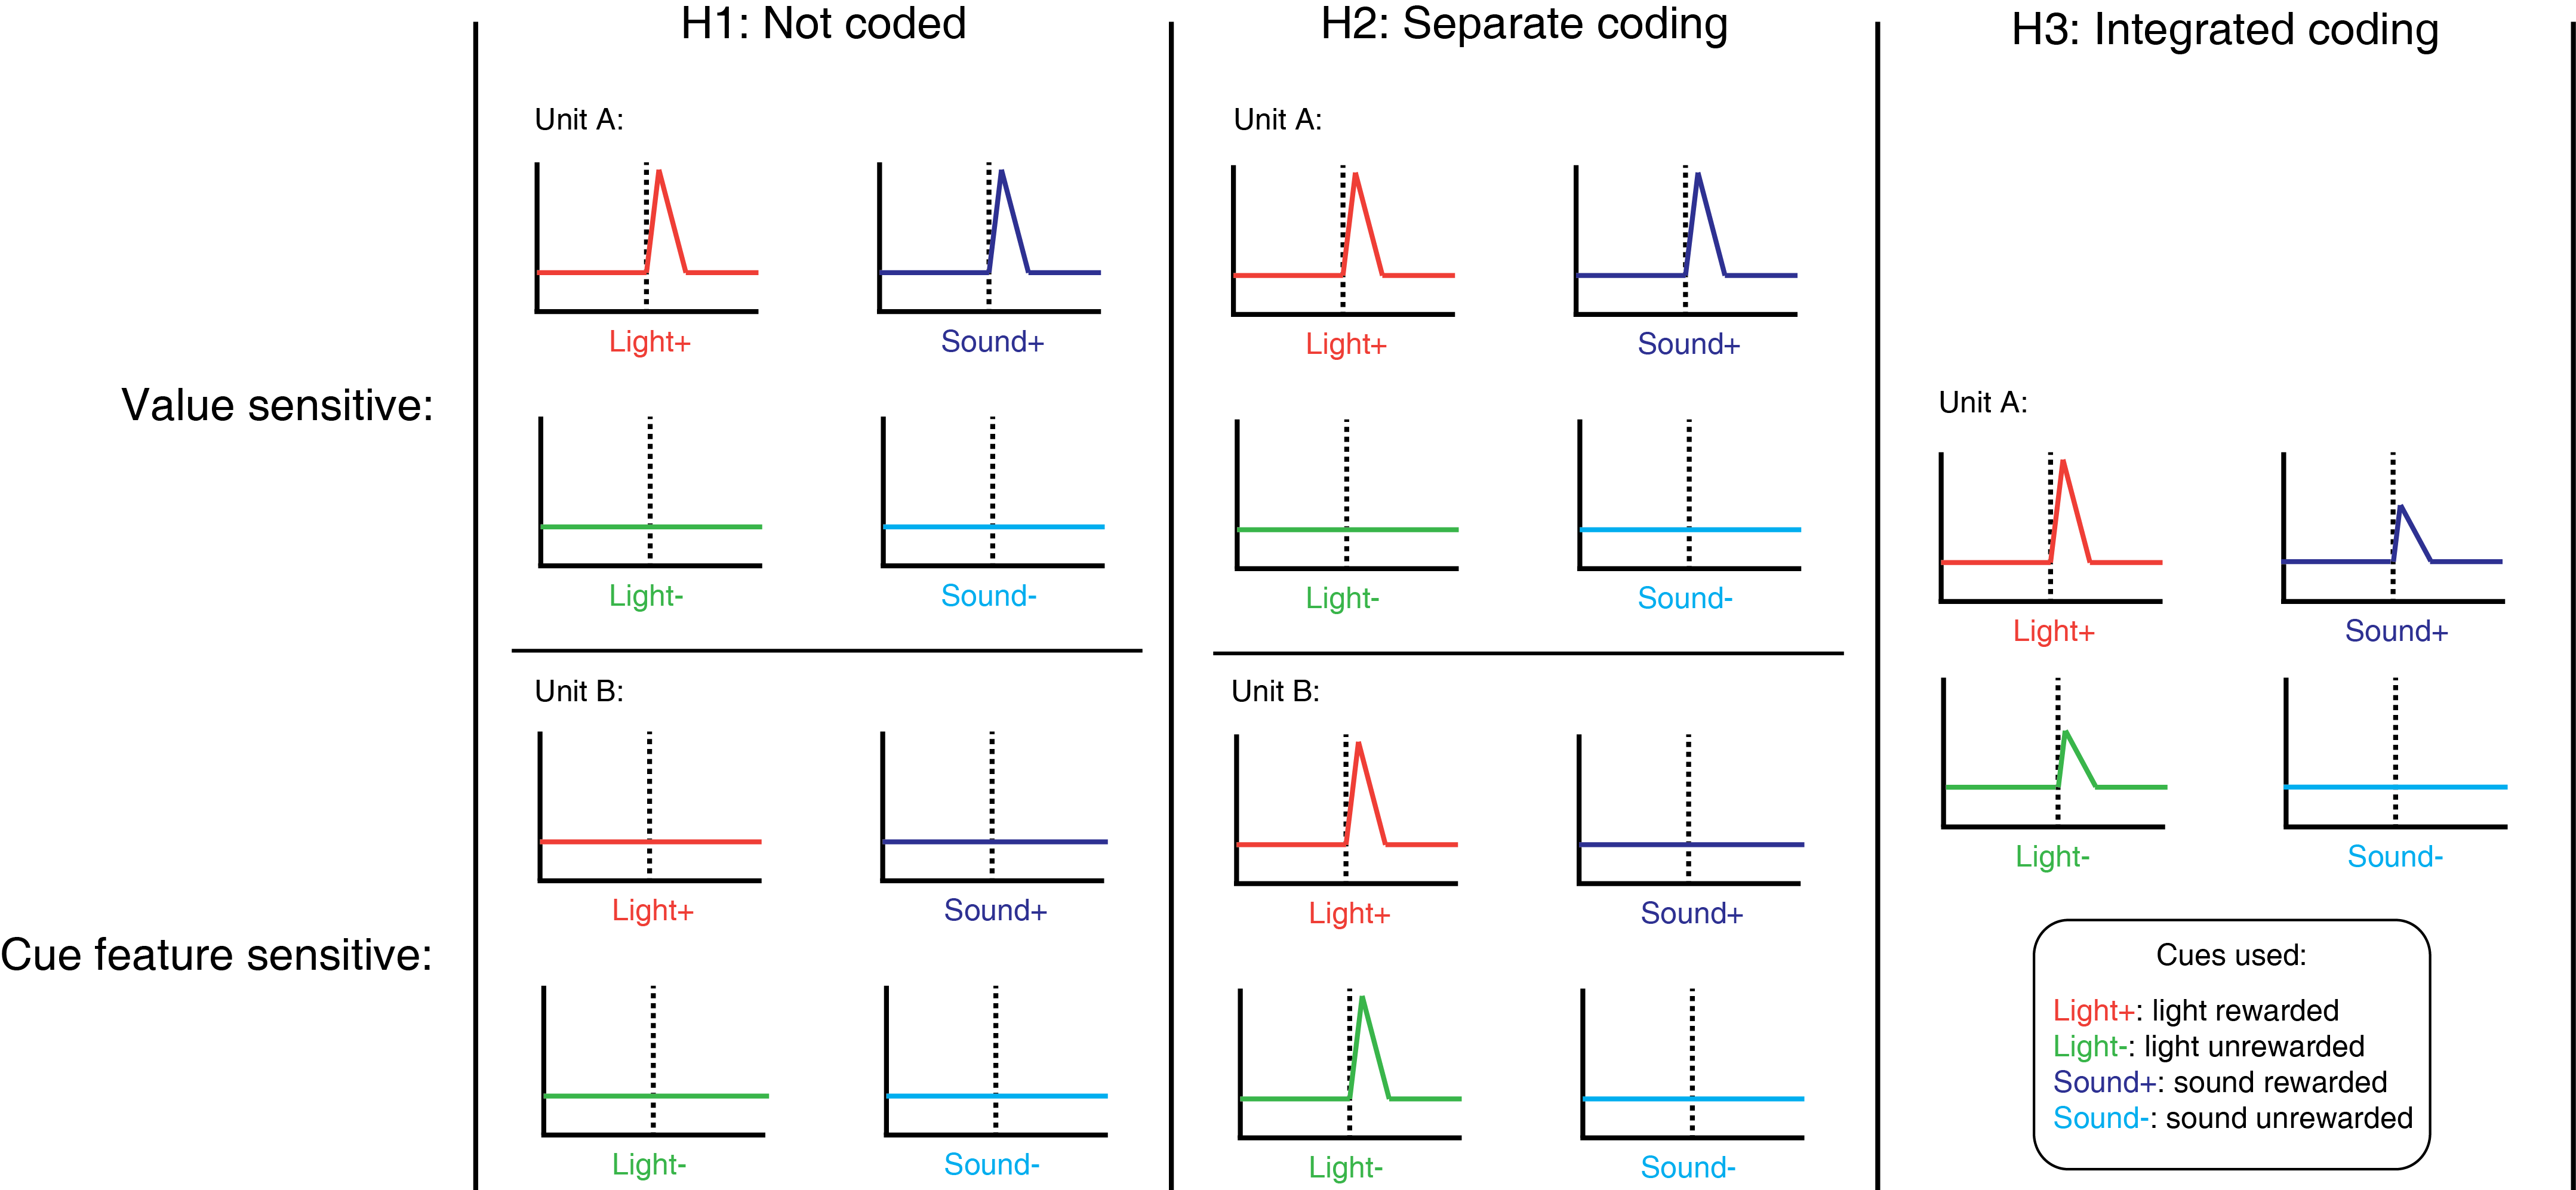
\includegraphics[width=\textwidth]{Fig 1 - Schematic neural.png}
\caption{Schematic of potential coding strategies employed by single units in the NAc. Aim 1. Displayed are schematic PETHs illustrating putative responses to different cues under different hypotheses of how cue identity and value are coded. H1 (left panel): Coding of cue identity is absent in the NAc. Top: Unit A responds to a motivationally relevant variable, such as expected outcome, similarly across other cue features, such as stimulus modality or physical location. Hypothetical plot is firing rate across time. Light+ (red) signifies a reward-available light cue, Sound+ (navy blue) a reward-available sound cue, Light- (green) a reward-unavailable light cue, Sound- (light blue) a reward-unavailable sound cue. Dashed line indicates onset of cue. Bottom: No units within the NAc discriminate their firing according to cue identity. H2 (middle panel): Coding of cue identity occurs independently of encoding of motivationally relevant variables like expected outcome or subsequent vigor. Top: Same as H1, with unit A discriminating between reward-available and reward-unavailable cues. Bottom: Unit B discriminates firing across stimulus modalities, depicted here as firing to light cues but not sound cues. H3 (right panel): Coding of cue identity is integrated with coding of other motivationally relevant variables. Hypothetical example demonstrating a unit that responds to reward-predictive cues, but firing rate is also modulated by stimulus modality, firing most for the reward-available light cue. Aim 2. Displayed are schematic PETHs illustrating potential ways in which cue identity is represented. H1 (left panel): Cue-onset triggers a transient response to a unit that codes for cue identity. Dashed lines indicate time of a behavioral or environmental event. ‘Cue-ON’ signifies onset of cue, ‘NP’ signifies when the rat holds a nosepoke at a reward receptacle, ‘Out’ signifies when the outcome is revealed, ‘Cue-OFF’ signifies when the cue turns off. H2 (middle panel): Coding of cue identity is maintained during a nosepoke hold period until outcome is revealed. H3 (right panel): Coding of cue identity is maintained during entire duration of cue, including after outcome is revealed. Same hypotheses applies to other information-containing aspects of the environment when the cue is presented, such as the physical location of the cue.}
\label{fig:schematic}
\end{figure}

\section*{Methods}

{\bf Subjects:}

Adult male Long-Evans rats (n = 4, Charles River, Saint Constant, QC) were used as subjects. Rats were individually housed with a 12/12-h light-dark cycle, and tested during the light cycle. Rats were food deprived to 85-90\% of their free feeding weight (weight at time of implantation was 440 - 470 g), and water restricted 4-6 hours before testing. All experimental procedures were approved by the the University of Waterloo Animal Care Committee (protocol\# 11-06) and carried out in accordance with Canadian Council for Animal Care (CCAC) guidelines.

{\bf Overall timeline:}

Each subject was first handled for seven days during which they were exposed to the running room, the sucrose solution used as a reinforcer, and the click of the valves upon approach to the receptacles. They were then shaped to run on the task for seven days where they were restricted to running in the clockwise direction by presenting a physical barrier to running counterclockwise. Rats then continued to be trained each day for 100 trials in both a light and sound block until approach behavior discriminated between reward-available and reward-unavailable cues for three consecutive days according to a chi square test, at which point they underwent hyperdrive implantation targeted at the NAc. Rats were allowed to recover for a minimum of five days before being retrained on the task, and recording began once performance returned to pre-surgery levels. Upon completion of recording, animals were sacrificed and recording sites were histologically confirmed.

{\bf Behavioral task and training:}

Rats were trained to run clockwise on an elevated, square-shaped track (100x100 cm) containing four possible reward locations (Figure \ref{fig:task}). Rats initiated a trial by running down the length of an arm, and triggering a photobeam located 24 cm from the start of each arm. Upon trial initiation, a light or sound cue was presented that signaled the presence (reward-available trial) or absence (reward-unavailable trial) of a 12\% sucrose water reward (0.1 mL) at the upcoming site. A trial was classified as an approach trial if the rat turned left at the decision point and made a nosepoke at the reward receptacle (40 cm from the decision point), while trials were classified as a skip trial if the rat instead turned right at the decision point and triggered the photobeam to initiate the following trial. In reward-available trials there was a 1 second delay between a nosepoke and subsequent reward delivery. Trial length was determined by measuring the length of time from cue onset until nosepoke (for approach trials), or from cue onset until the start of the following trial (for skip trials). Trials could only be initiated through clockwise progression through the series of arms, and each entry into the subsequent arm on the track counted as a trial. To get enough trials for neural analysis rats were trained each day in both a light and sound block for 100 trials each. Within a block, one cue signaled reward was available on that trial, while the other signaled reward was not available. Light block cues were a flashing white light, and a constant yellow light. Sound block cues were a 2 kHz sine wave and a 8 kHz sine wave whose amplitude was modulated from 0 to maximum by a 2 Hz sine wave. Reward-cue associations were counterbalanced across rats. Cue presentation was pseudorandomized so that the same cue could not be presented more than twice in a row. Block order within each day was also pseudorandomized, such that the rat could begin a session with the same block for more than two days in a row. Each training or testing day consisted of a 5 minute pre-session period on a pedestal, followed by the first block, then the second block, then a 5 minute post-session period on the pedestal. Performance was determined by the proportion of trials a rat approached each cue. Perfect performance would be 100\% approach on reward-available trials, and 0\% approach on reward-unavailable trials. Rats were trained daily until they could distinguish between the reward-available and reward-unavailable cues for both light and sound blocks for three consecutive days, according to a chi-square test rejecting the null hypothesis of equal approaches for reward-available and reward-unavailable trials, at which point they underwent surgery. 

\begin{figure}[h]
\centering
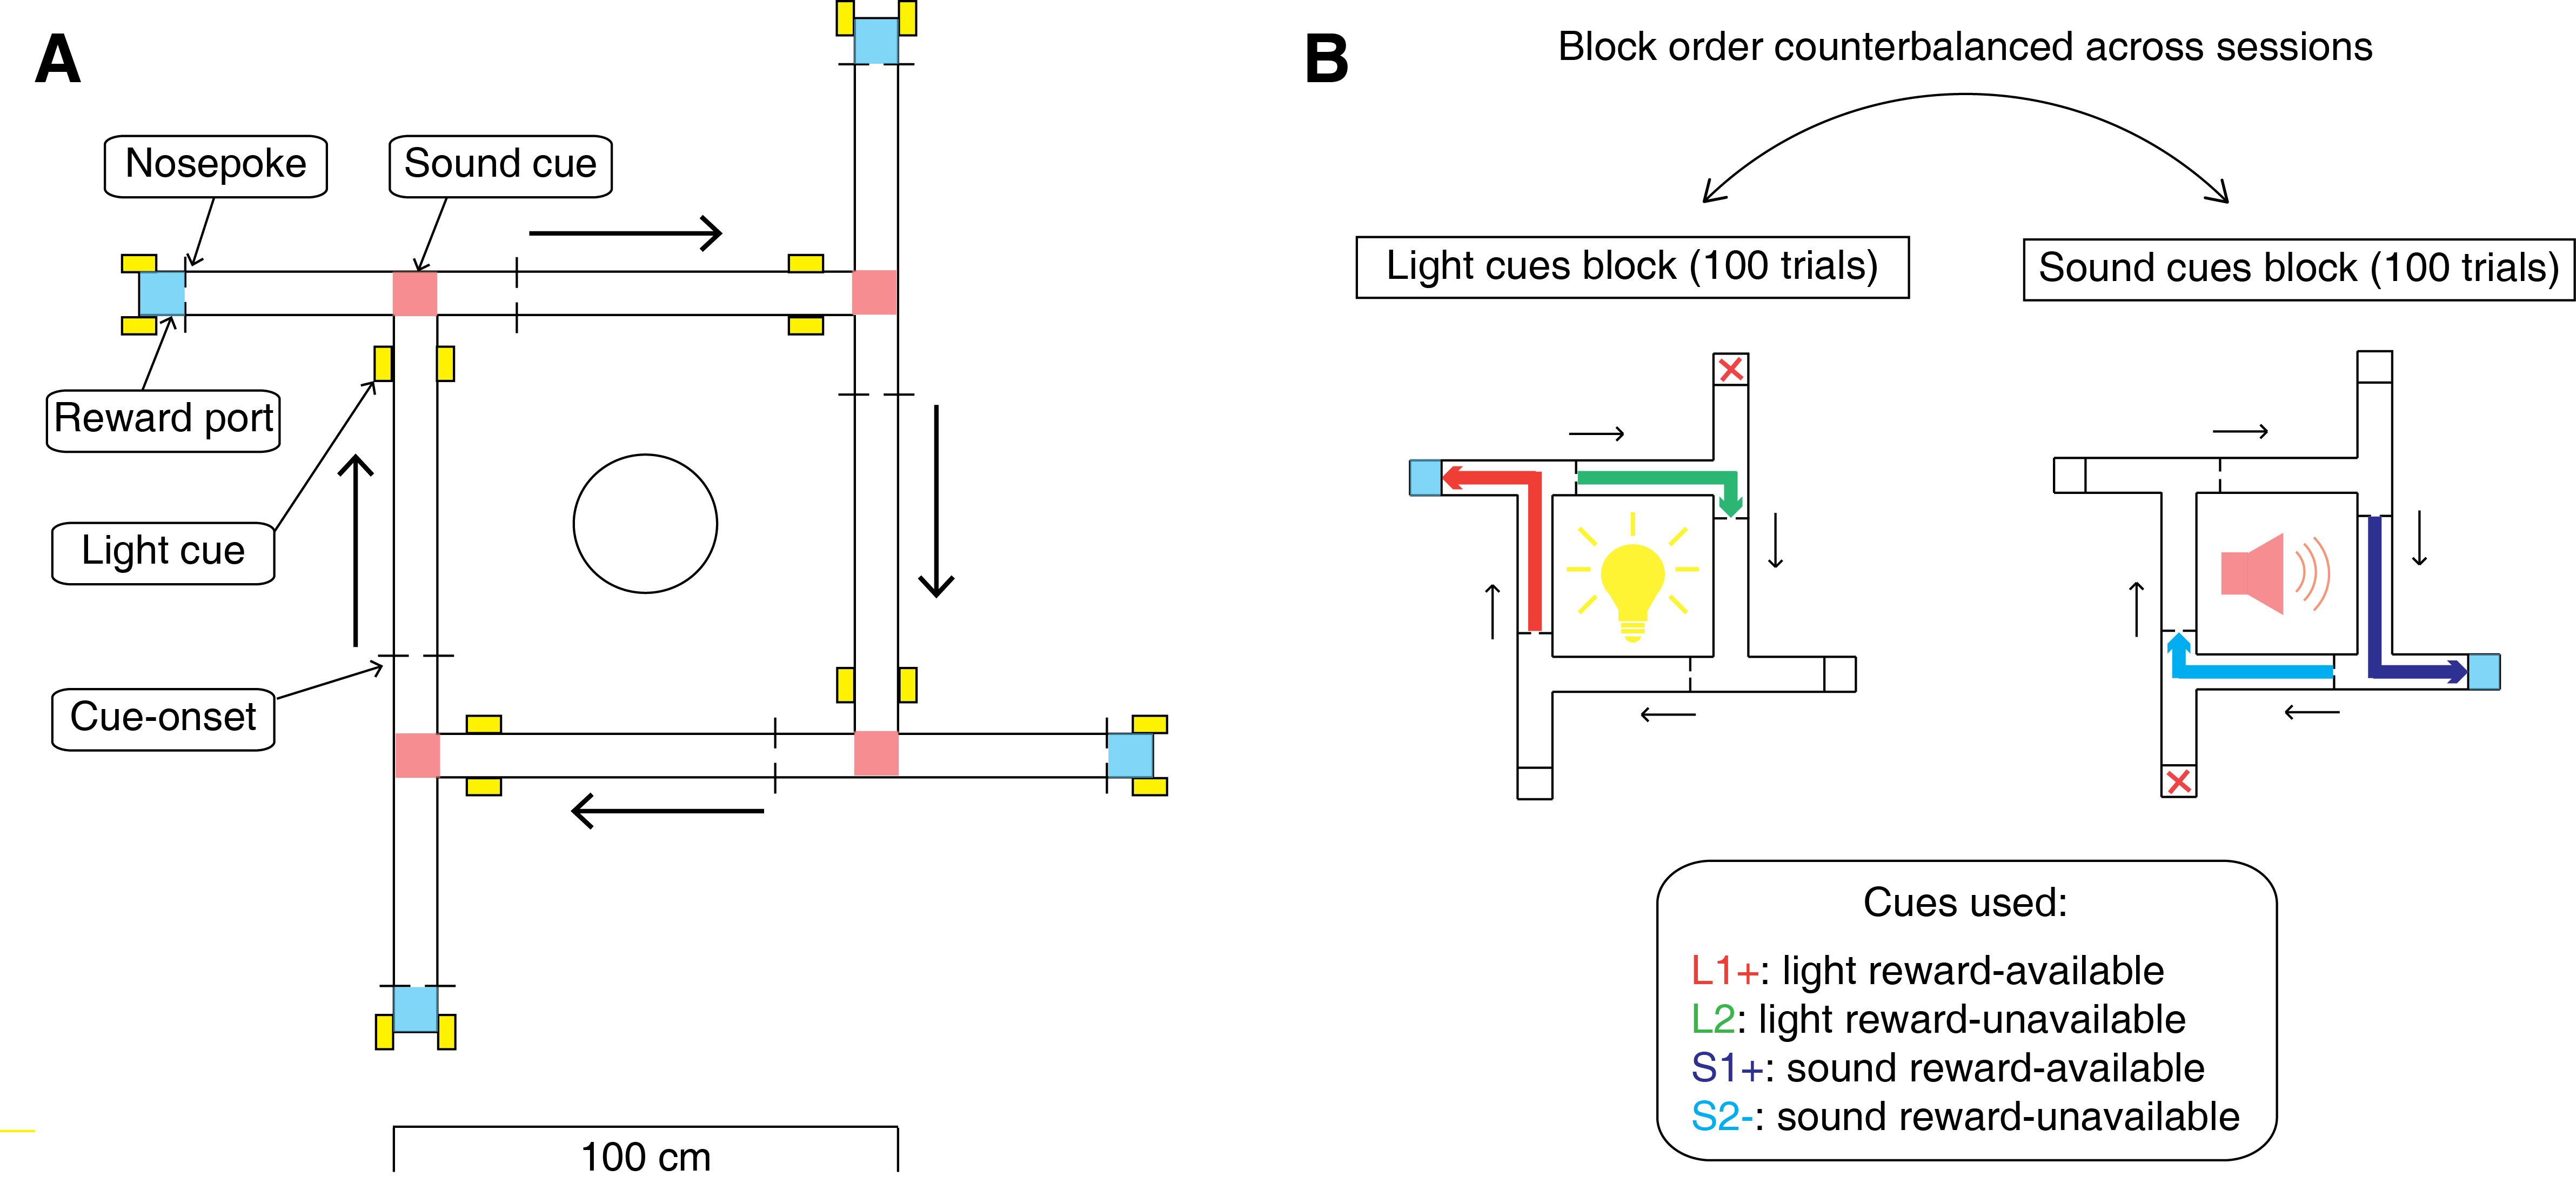
\includegraphics[width=\textwidth]{Fig 2 - Schematic task.png}
\caption{Schematic of behavioral task. A. To scale depiction of square track consisting of multiple identical T-choice points. Dashed lines indicate location of photobeams. Photobeams on the center, square portion of the track triggered the start of a trial and onset of a cue, whereas photobeams at the ends of the arms by the receptacles registered nosepokes. Rectangular boxes with yellow fill indicate location of LEDs used for light cues. Speakers for tone cues were placed underneath the choice points, indicated by magenta fill on track. Light blue fill on ends of arms indicate location of receptacles where sucrose was dispensed on rewarded trials. Circle in the center indicates location of pedestal during pre- and post-records. Scale bar is located beneath the track. B. Progression of a recording session. A session was started with a 5 minute recording period on a pedestal placed in the center of the apparatus. Rats then performed two blocks of a cue discrimination task on a square track where they had to dissociate between a reward-available and reward-unavailable cue for a set of light cues and a set of sound cues for a target of 100 trials each. Rats ran clockwise on the square track, and upon presentation of the cue could either turn left at the choice point to check if reward was available at the reward receptacle (approach trial; red and navy blue in figure), or turn right at the choice point to initiate the following trial (skip trial; green and light blue in figure). Reward-available and reward-unavailable cues were presented pseudo-randomly, such that not more than two of the same type of cue could be presented in a row. Location of the cue on the track was irrelevant for behavior, all cue locations contained an equal amount of reward-available and reward-unavailable trials. Left in figure depicts a light block, showing an example trajectory for a correct reward-available (red) and reward-unavailable (green) trial. Right in figure depicts a sound block, with a reward-available (navy blue) and reward-unavailable (light blue) trial. Ordering of the light and sound blocks was counterbalanced across sessions. Dashed line within track indicates photobeam that triggered cue onset. Solid line within track indicates photobeam that registered a nosepoke into the reward receptacles. Receptacles containing sucrose solution are present within the squares at the end of each arm. Light blue fill signifies reward receipt on a correct reward-available trial. Arrows outside of track indicate correct running direction. A session ended with another 5 minute recording period on the pedestal.}
\label{fig:task}
\end{figure}

{\bf Surgery:}

Surgical procedures were as described previously (Malhotra et al., 2015). Briefly, animals were anesthetized with isoflurane, induced with 5\% in medical grade oxygen and maintained at 2\% throughout the surgery (~0.8 L/min). Rats were then chronically implanted with a “hyperdrive” consisting of 16 independently drivable tetrodes, either all 16 targeted for the right NAc (AP +1.4 mm and ML +1.6 mm, relative to bregma; Paxinos and Watson, 2005), or 12 in the right NAc and 4 targeted at the mPFC (AP +3.0 mm and ML +0.6 mm, relative to bregma; only data from NAc tetrodes were analyzed). Following surgery, all animals were given at least five days to recover and lower tetrodes to the target (DV -6.0 mm) before being reintroduced to the behavioral task.

{\bf Data acquisition and preprocessing:}

After recovery, rats were placed back on the task for recording. NAc signals were acquired at 20 kHz with a RHA2132 v0810 preamplifier (Intan) and a KJE-1001/KJD-1000 data acquisition system (Amplipex). Signals were referenced against a tetrode placed in the corpus callosum above the NAc.

Candidate spikes for sorting into putative single units were obtained by band-pass filtering the data between 600-9000 Hz, thresholding and aligning the peaks (UltraMegaSort2k, Hull et al., 2011). Spike waveforms were then clustered with KlustaKwik using energy and the first derivative of energy as features, and manually sorted into units (MClust 3.5, A.D. Redish et al.). Isolated units containing a minimum of 200 spikes within a session were included for subsequent analysis. Units were classified as fast spiking interneurons (FSIs) by an absence of interspike intervals (ISIs) $>$ 2 s, while medium spiny neurons (MSNs) had a combination of ISIs $>$ 2 s and phasic activity with shorter ISIs (Barnes 2005, Atallah 2014).

{\bf Data analysis:}

For behavioral performance we generated linear mixed effects models to investigate the relationships between cue type and our behavioral variables, with cue type as a fixed effect, and the addition of an intercept for rat identity as a random effect. Average proportion of trials approached and trial length for a session were used as response variables. Contribution of cue type to behavior was determined by comparing the full model to a model with cue type removed for each behavioral variable.

To investigate the contribution of various cue features on NAc firing rates we first determined whether firing rates for a unit were modulated by the onset of a cue by collapsing across all cues and comparing the firing rates for the 1 s preceding cue-onset with the 1 s following cue-onset. Single units were considered to be cue-responsive if a Wilcoxon signed-rank test comparing pre- and post-cue firing had a p $<$ .01. (Excluded: ‘the mean firing rate difference between pre- and post-cue onset was within the lower or upper 2.5\% of a shuffled distribution’, as there is redundancy using both, and I did both because I was paranoid about just using one. ). Cue-modulated units were then classified as either increasing or decreasing in response to the cue if the post-cue activity was higher or lower than the pre-cue activity, respectively.

To determine the relative contribution of various task parameters to firing rate variance for units whose firing was modulated by cue-onset (as in Figures \ref{fig:examples},\ref{fig:GLM}), a forward selection stepwise general linear model (GLM) was fit to each cue-responsive unit. Cue identity (light block, sound block), cue location (arm 1, arm 2, arm 3, arm 4), cue outcome (reward-available, reward-unavailable), approach behavior, trial length, trial number, and trial history were used as predictors, and the 1 s post-cue firing rate as the response variable. Units were classified as being modulated by a given task parameter if addition of the parameter significantly improved model fit using deviance as the criterion (p $<$ .01). A comparison of the R-squared value between the final model and the final model minus the predictor of interest was used to determine the amount of firing rate variance explained by the addition of that predictor for a given unit.

To better visualize responses to cues and enable subsequent population level analyses (as in Figures \ref{fig:examples},\ref{fig:pop},\ref{fig:tiling}), spike trains were convolved with a Gaussian kernel ($\sigma$ = 100 ms), and peri-event time histograms (PETHs) were generated by taking the average of the convolved spike trains across trials for a given task condition. For analysis of population-level responses for cue features (Figure \ref{fig:pop}), convolved spike trains for all units where cue identity, cue location, or cue outcome explained a significant portion of firing rate variance were z-scored. Within a given cue feature, normalized spike trains were then separated according to the preferred and non-preferred cue condition (e.g. light vs sound block), and averaged across units to generate population-level averages.

To visualize NAc representations of task space within cue conditions, normalized spike trains for all units were ordered by the location of their maximum or minimum firing rate for a specified cue condition (Figure \ref{fig:tiling}). To compare representations of task space across cue conditions for a cue feature, the ordering of units derived for one condition (e.g.\ light block) was then applied to the normalized spike trains for the other condition (e.g.\ sound block). For control comparisons within cue conditions, half of the trials for a condition were compared against the other half. To look at the correlation of firing rates of all cells within and across various cue conditions, trials for each cue condition for a cell were shuffled and divided into two averages, and averages within and across cue conditions were correlated. A linear mixed effects model was run for each cue condition to determine if correlations of firing rates within cue conditions were more similar than correlations across cue conditions.

To identify the responsivity of units to different cue features at the time of a nosepoke into a reward receptacle, and subsequent reward delivery, the same cue-responsive units from the cue-onset analyses were analyzed at the time of nosepoke and reward receipt using identical analysis techniques (Figures \ref{fig:NP_GLM},\ref{fig:NP_pop},\ref{fig:NP_tiling}).

Given that some of our analyses compare firing rates across time, particularly comparisons across blocks, we sought to exclude units with unstable firing rates that would generate spurious results reflecting a drift in firing rate over time unrelated to our task. To do this we ran a Mann-Whitney U test comparing the cue-evoked firing rates for the first and second half of trials within a block, and excluded 99 units from analysis that showed a significant change for either block. All analyses were completed in MATLAB R2015a, the code is available on our public GitHub repository (http://github.com/vandermeerlab/papers), and the data can be accessed through DataLad.

{\bf Histology:}

Upon completion of the experiment, rats were anesthetized with 5\% isoflurane, then asphyxiated with carbon dioxide. Transcardial perfusions were performed, and brains were fixed and removed. Brains were sliced in 50 $\mu m$ coronal sections and stained with thionin. Slices were visualized under light microscopy, tetrode placement was determined, and electrodes with recording locations in the NAc were analyzed (Figure \ref{fig:histo}).

\begin{figure}[h]
\centering
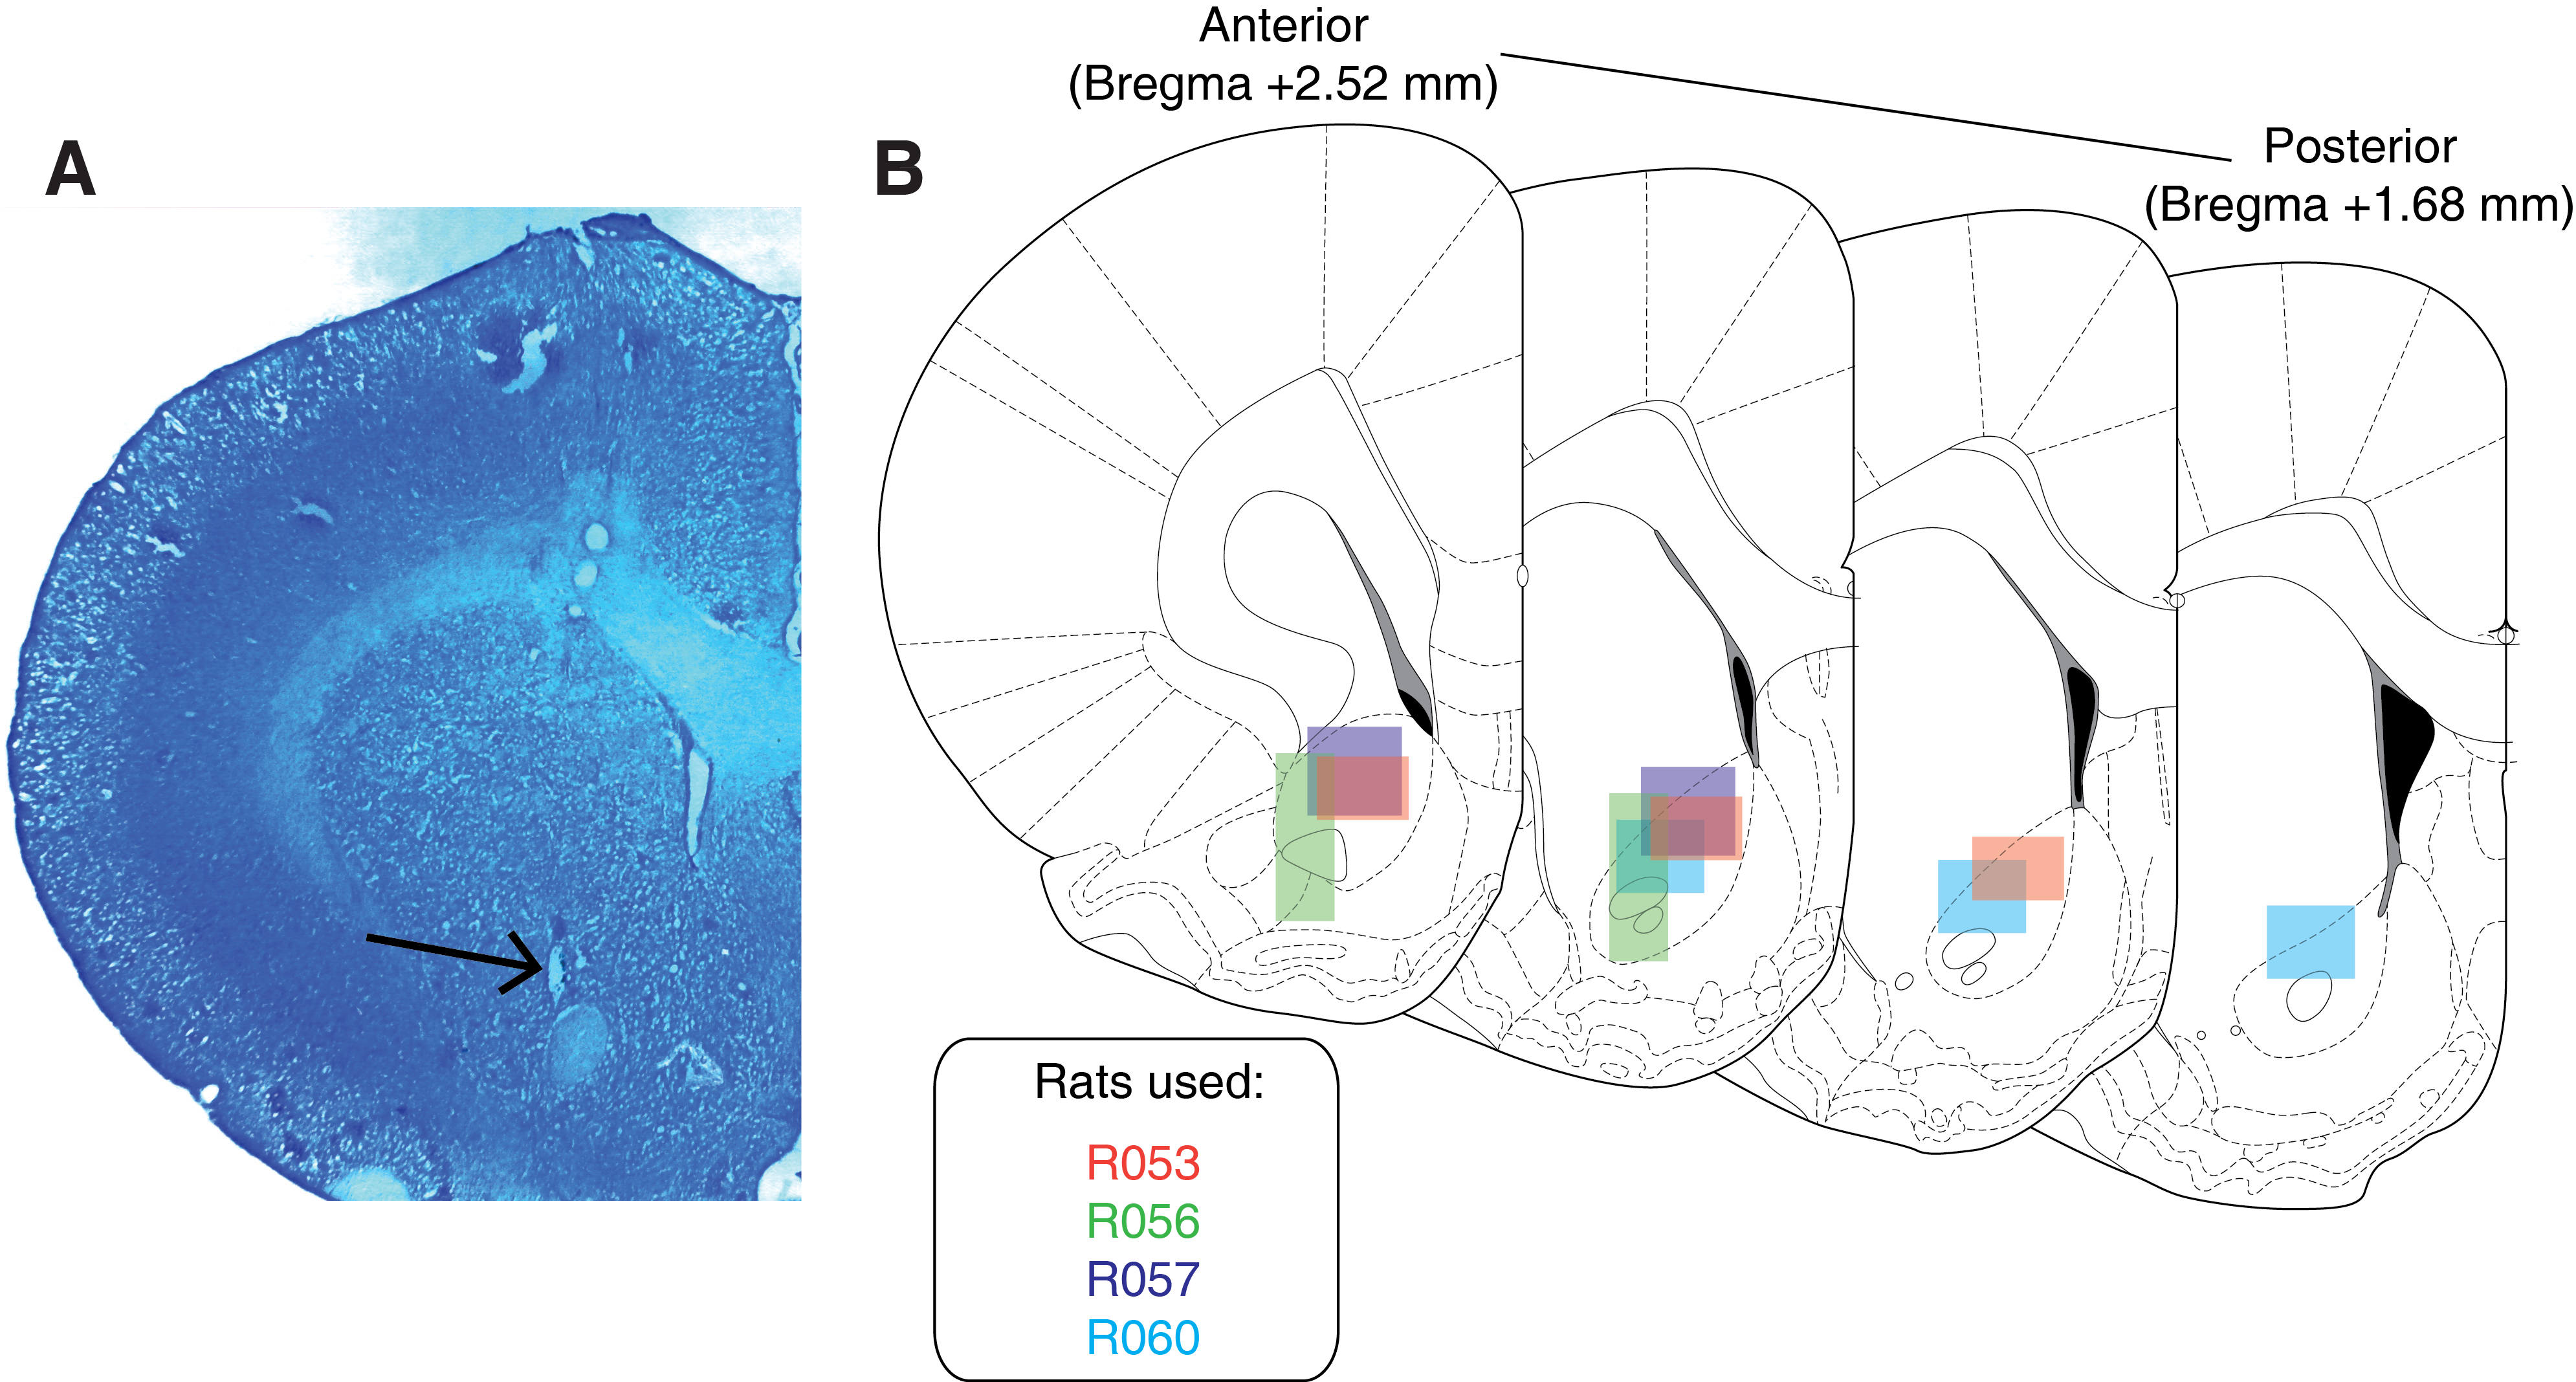
\includegraphics[width=\textwidth]{Fig 3 - Histology.png}
\caption{Histological verification of recording sites. Upon completion of experiments, brains were sectioned and tetrode placement was confirmed. A. Example section from R060 showing a recording site in the NAc core just dorsal to the anterior commissure (white circle). B. Schematic showing recording areas for the four rats used in the present study..}
\label{fig:histo}
\end{figure}

\section*{Results}

\subsection*{Behavior}

Rats were trained to discriminate between cues signaling the availability and absence of reward on a square track with four identical arms for two distinct sets of cues. During each session, rats were presented sequentially with two behavioral blocks containing cues from different sensory modalities, a light and a sound block, with each block containing a cue that signalled the availability of reward (reward-available), and a cue that signalled the absence of reward (reward-unavailable). An example learning curve is seen in Figure \ref{fig:behav}A,B. All four rats learned to discriminate between the reward-available and reward-unavailable cues for both the light and sound blocks as determined by reaching significance (p $<$ .05) on a daily chi-square test comparing approach behavior for reward-available and reward-unavailable cues for each block, for at least three consecutive days (range for time to criterion: 22 - 57 days). Maintenance of behavioral performance during recording sessions was assessed using linear mixed effects models for both proportion of trials where the rat approached the receptacle, and trial length. Analyses revealed that the likelihood of a rat to make an approach was influenced by which of the cues was presented (Percentage approached: light reward-available = 97\%; light reward-unavailable = 34\%; sound reward-available = 91\%; sound reward-unavailable 35\%; p $<$ .001), but that cue identity did not significantly affect the length of time taken to complete a trial (Trial length: light reward-available = 1.85 s; light reward-unavailable = 1.74 s; sound reward-available = 1.91 s; sound reward-unavailable 1.78 s; p $=$ .13)(Figure \ref{fig:behav}C,D). Thus, during recording, rats successfully discriminated the various cues according to whether or not they signalled the availability of reward at the reward receptacle.

\begin{figure}[h]
\centering
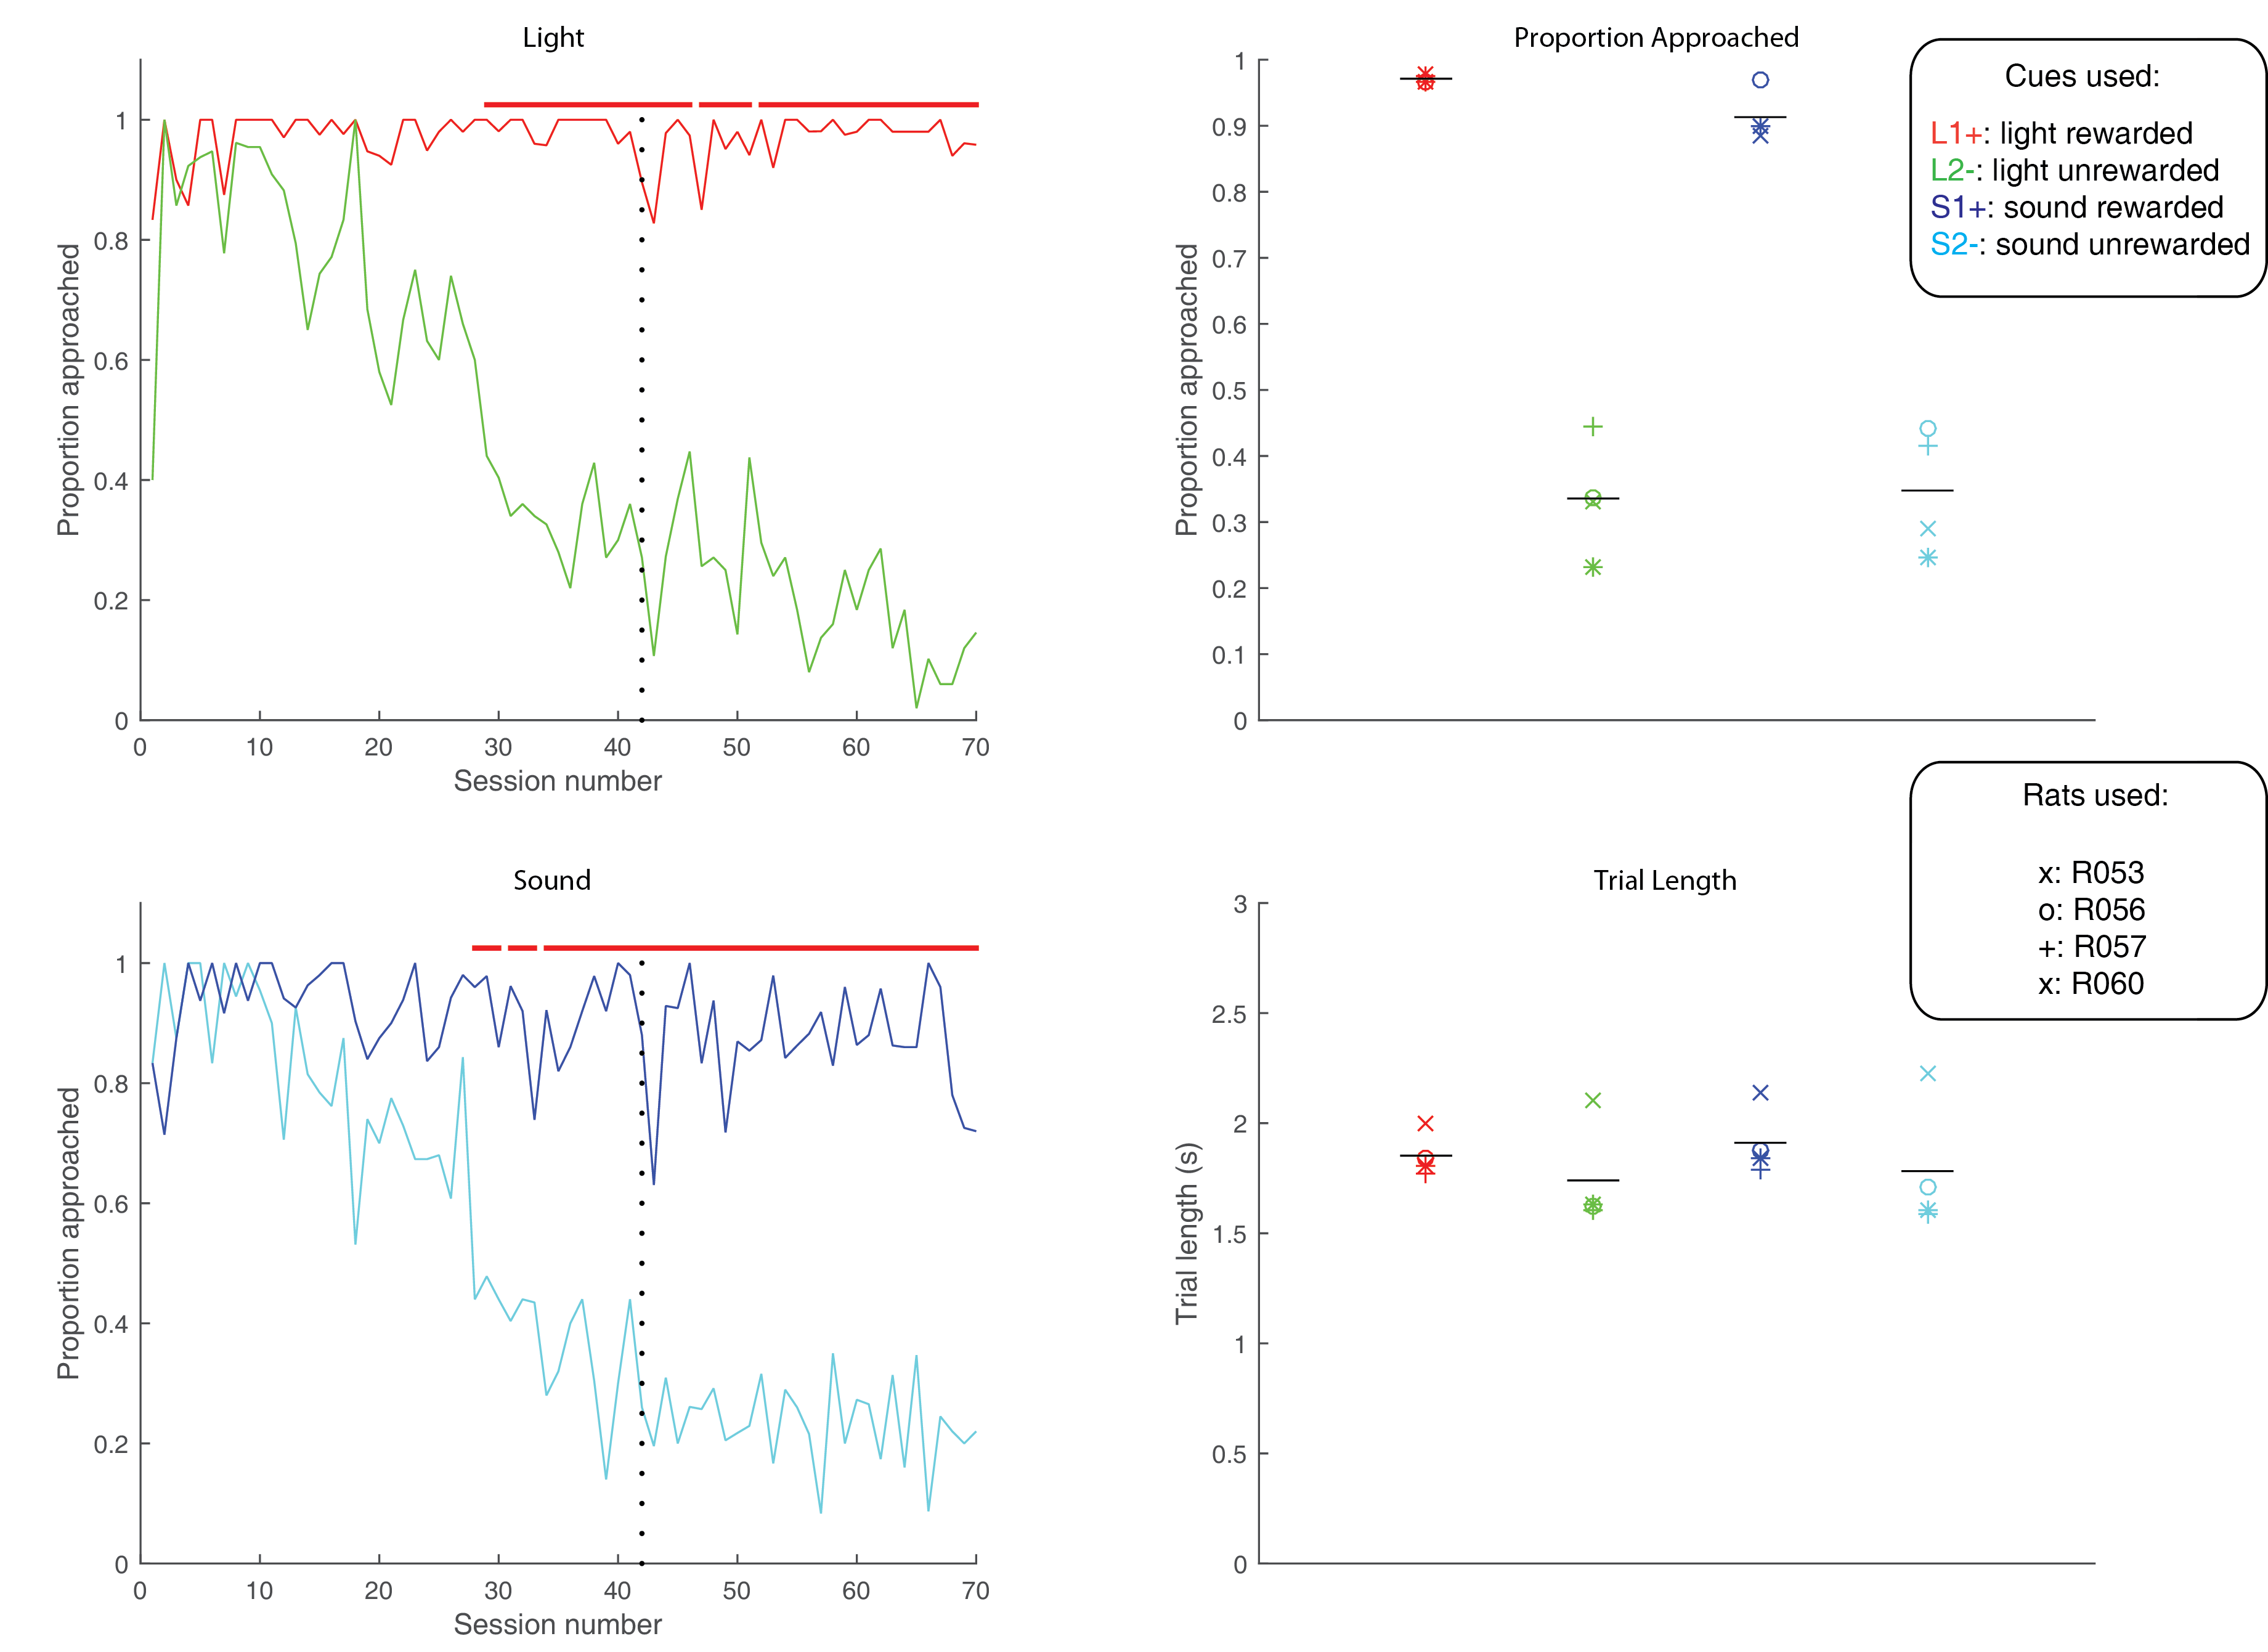
\includegraphics[width=\textwidth]{Fig 4 - Behavioral results.png}
\caption{Performance on the behavioral task. A-B. Example learning curves across sessions from a single subject (R060) showing the proportion approached for reward-available (red line for light block, navy blue line for sound block) and reward-unavailable trials (green line for light block, light blue line for sound block). Fully correct performance corresponds to approach proportion of 1 for reward-available trials and 0 for reward-unavailable trials. Rats initially start out approaching on both reward-available and reward-unavailable trials, and learn with experience to skip non-rewarded trials. Red bars indicate days in which a rat statistically discriminated between reward-available and reward-unavailable cues, determined by a chi square test. Dashed line indicates time of electrode implant surgery. C-D. Summary of performance during recording sessions for each rat. C. Proportion approached for all rats, averaged across all recording sessions. Different columns indicate the different cues (reward-available (red) and reward-unavailable (green) light cues, reward-available (navy blue) and reward-unavailable (light blue) sound cues). Different symbols correspond to individual subjects; horizontal black line shows the mean. All rats learned to discriminate between reward-available and reward-unavailable cues, as indicated by the clear difference of proportion approached between reward-available ($\sim$90\% approached) and reward-unavailable cues ($\sim$30\% approached), for both blocks (see Results for statistics). D. Average trial length for each cue. Note that the time to complete a trial was comparable for the different cues.}
\label{fig:behav}
\end{figure}

\subsection*{NAc neurons encode behaviorally relevant and irrelevant cue features}

{\bf Single unit responses discriminate cue features:}

We sought to address which parameters of our task were encoded by NAc activity, specifically whether the NAc encodes aspects of motivationally relevant cues not directly tied to reward, such as the identity and location of the cue, and whether this coding is independent or integrated with coding of cue outcome. To do this we recorded a total of 443 units with $>$ 200 spikes in the NAc from 4 rats over 57 sessions while they performed a cue discrimination task (Table \ref{tbl1}). Units that exhibited a drift in firing rate over the course of either block were excluded from further analysis, leaving 344 units for further analysis. The activity of 128 (37\%) of these 344 units were modulated by the cue, with more showing a decrease in firing (n =  98) than an increase (n = 30) around the time of cue-onset (Table \ref{tbl2}). Within this group, 24 were classified as FSIs, while 104 were classified as SPNs. Upon visual inspection, we observed several patterns of firing activity, including units that; discriminated firing upon cue-onset across various cue conditions, showed sustained differences in firing across cue conditions, had transient responses to the cue, showed a ramping of activity starting at cue-onset, and showed elevated activity immediately preceding cue-onset, for example (Figure \ref{fig:examples}). To characterize more formally whether these cue-evoked responses were modulated by various aspects of the task, we fit a GLM to each cue-modulated unit. Fitting GLMs revealed that a variety of task parameters accounted for a significant portion of firing rate variance in NAc cue-modulated units (Figure \ref{fig:GLM}, Table \ref{tbl2}). Notably, there were units that discriminated between whether the rat was performing in the light or sound block (29\% of cue-modulated units, accounting for 6\% of variance on average), which arm the rat was currently on (39\% of cue-modulated units, accounting for 6\% of variance on average), and whether the rat was engaged in the common portion of a reward-available or reward-unavailable trial (27\% of cue-modulated units, accounting for 4\% of variance on average), suggesting that the NAc independently encodes features of reward-predictive cues separate from expected outcome (Figure \ref{fig:examples}A-F). Furthermore, interactions between multiple cue features appeared as significant predictors of firing rate variance for 9\% of cue-modulated units, although this effect was modest ($\sim$1-2\% variance explained), suggesting a weak effect for integrated coding across various aspects of a cue (Figure \ref{fig:examples}G,H). Fitting a GLM to all recorded units...*Jimmie finish this* (data not shown). Together, these findings show that various cue features are represented in the NAc, and that this coding has some overlap, but is mostly distinct from expected outcome (Figure \ref{fig:schematic}; H2,H3).

\begin{table}[p]
\centering
\setlength{\tabcolsep}{1 em} % for the horizontal padding
\begin{tabular}{l c  c c c c}

Rat                                  & Total        & MSN (increasing)        & MSN (decreasing)        &FSI (increasing)        &FSI (decreasing)\\
\hline
R053                       & 145         & 51          & 79          & 4         & 11\\
\hline
R056                       & 70         & 12          & 13         & 17          & 28\\
\hline
R057   	          & 136         & 55          & 75          & 3          & 3\\
\hline
R060                       & 92         & 37          & 49          & 3          & 3\\
\hline   

\end{tabular}
\caption {Cells from each rat} \label{tbl1} 
\end{table}

\begin{table}[p]
\centering
\setlength{\tabcolsep}{1 em} % for the horizontal padding
\begin{tabular}{l c  c c c c}

Task parameter                                 & Total        & MSN (increasing)        & MSN (decreasing)        &FSI (increasing)        &FSI (decreasing)\\
\hline
All cells                       & 443        & 155         & 216          & 27          & 45\\
\hline
Cue modulated                       & 128         &24          &80          & 6          &18\\
\hline
Cue identity       & 37         & 7          & 21          & 1          & 8\\
\hline
Cue location       & 50         &13          & 27          & 3          & 7\\
\hline
Cue outcome       & 34         & 10          & 18        & 0          & 6\\
\hline
Approach behavior      & 31         & 8          & 18          & 1          & 4\\
\hline
Trial length       & 25        & 5          & 18         & 0         & 2\\
\hline
Trial number       & 32         & 11          & 12         & 1          & 8\\
\hline
Recent trial history       & 5         & 0          &5          & 0          & 0\\
\hline
Cue x cue interactions       & 11         & 3          & 7          & 0          & 1\\
\hline
Cue x behavior interactions       & ?         & ?          & ?          & ?          & ?\\
\hline

\end{tabular}
\caption {Cells from GLM} \label{tbl2} 
\end{table}

\begin{figure}[h]
\centering
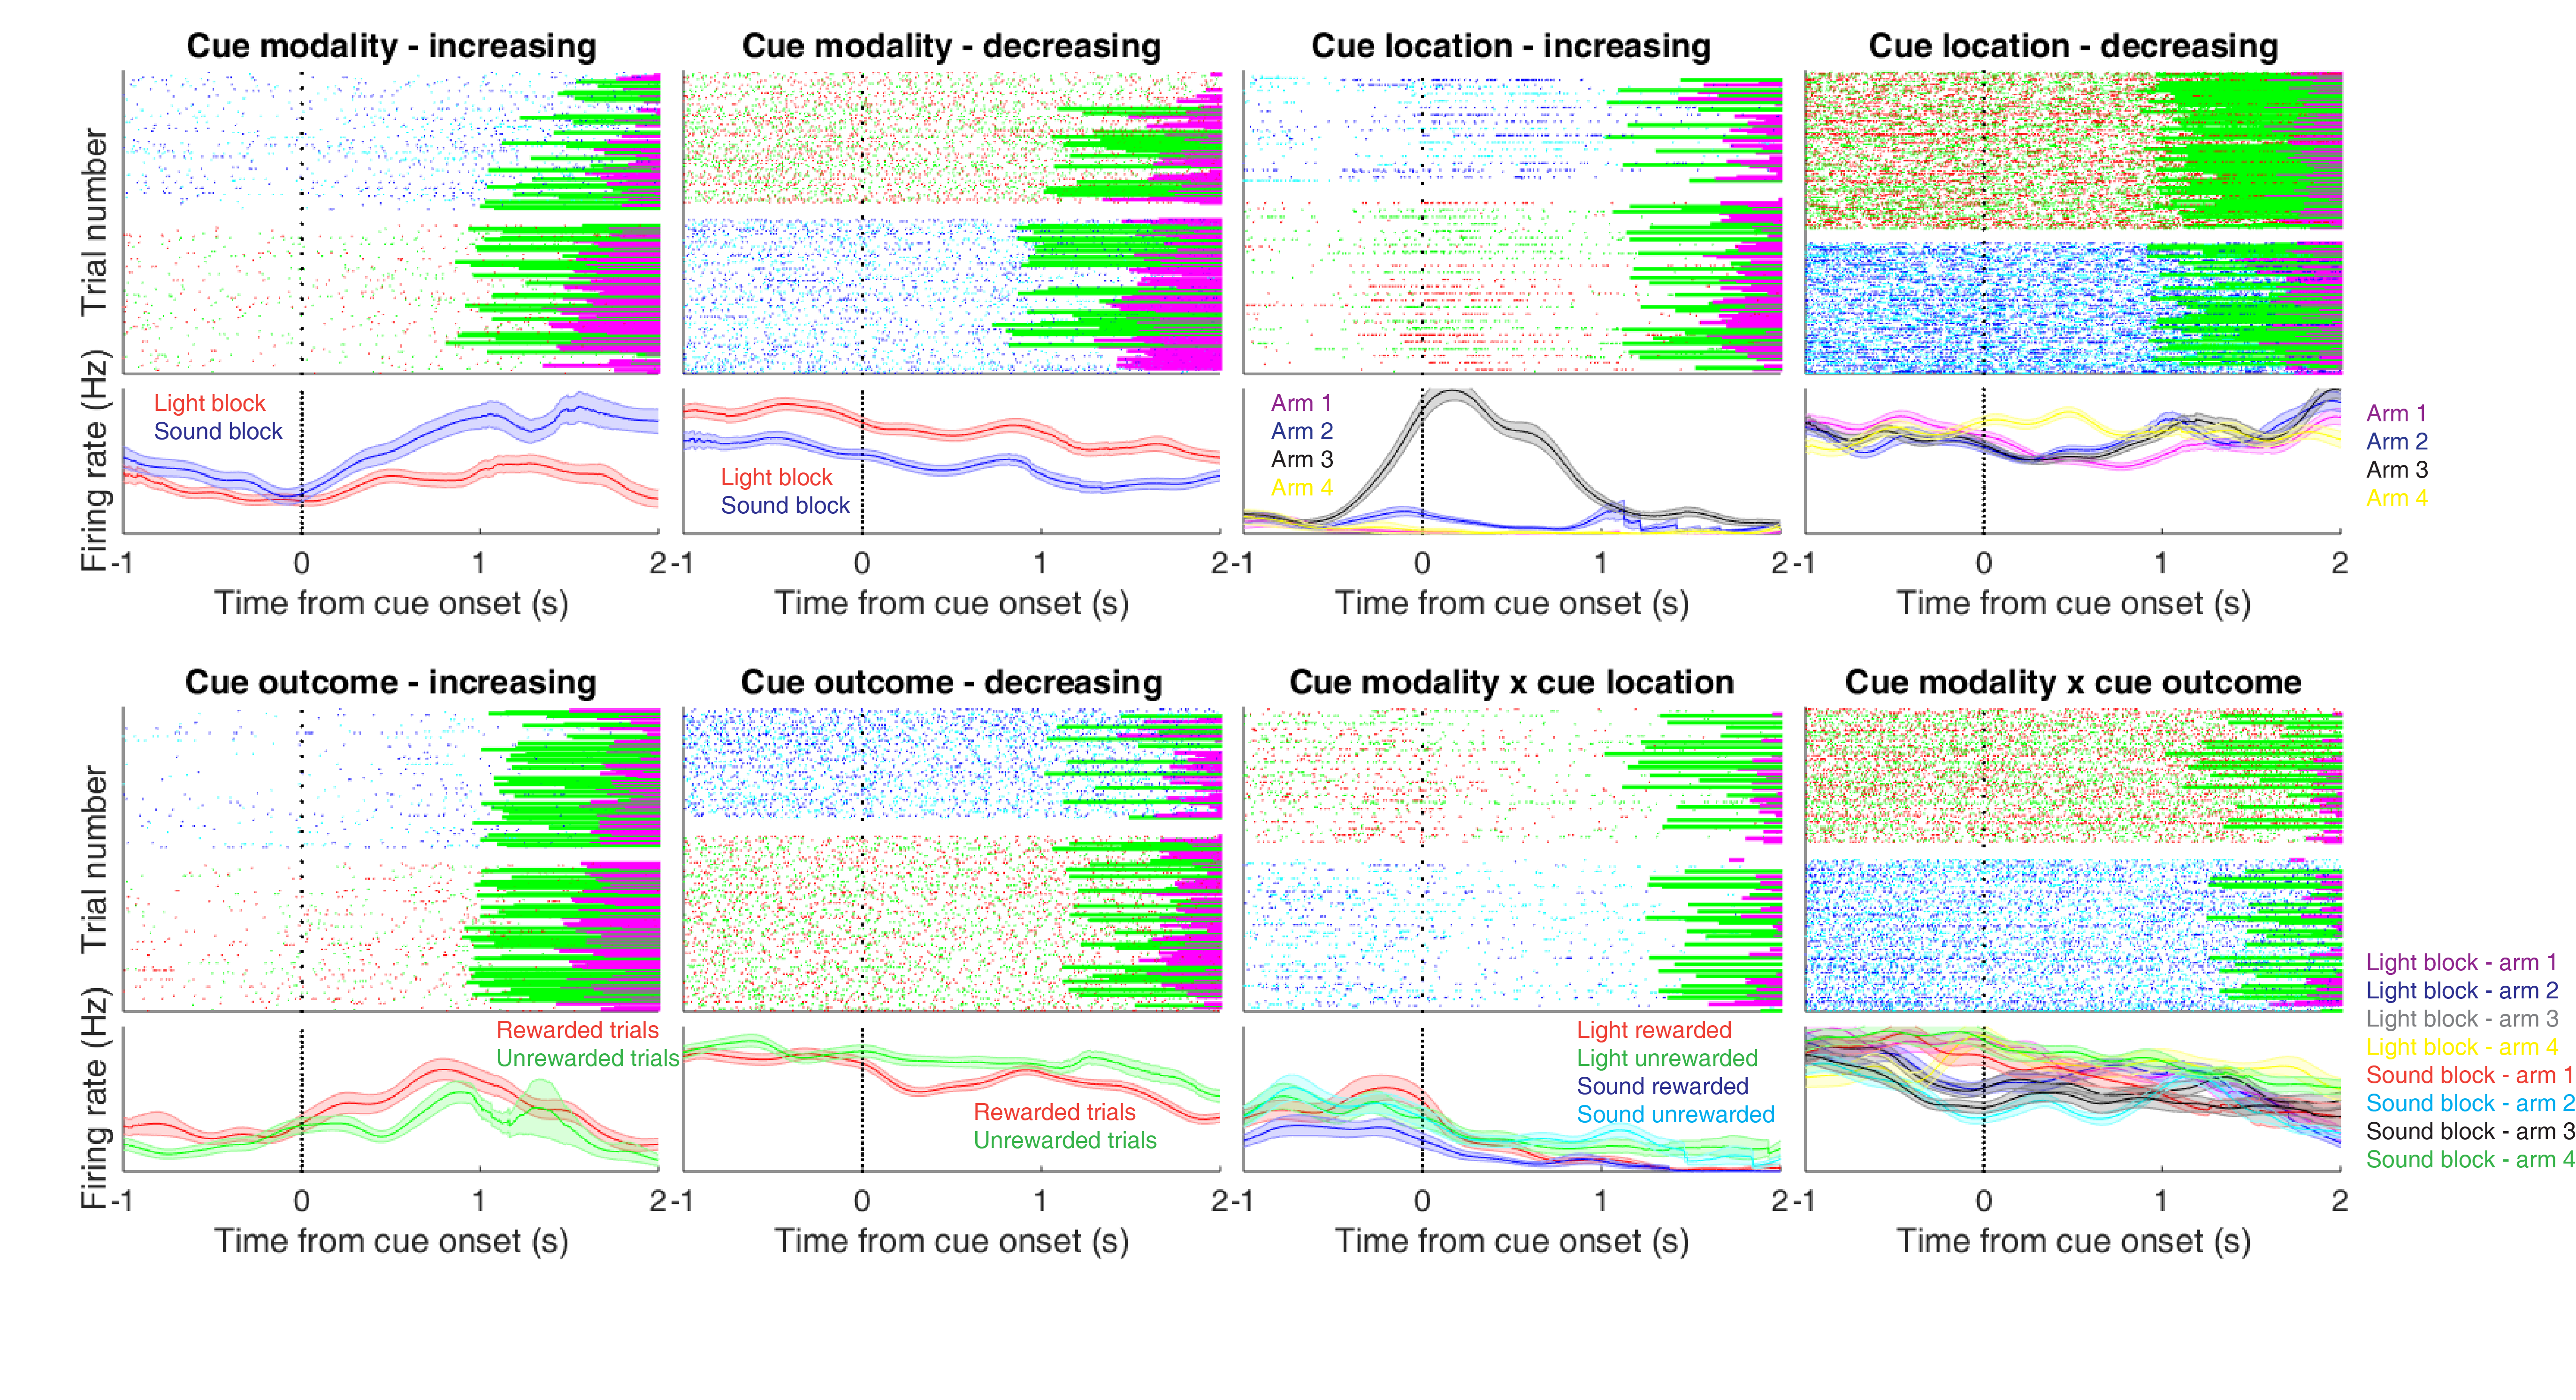
\includegraphics[width=\textwidth]{Fig 5 - Neural examples.png}
\caption{Examples of different cue-modulated NAc units influenced by various task parameters. A. Example of a cue-modulated NAc unit that showed an increase in firing in response to the cue, and encoded cue identity. Top: rasterplot showing the spiking activity across all trials aligned to cue-onset. Spikes across trials are color coded according to cue type (red: reward-available light; green: reward-unavailable light; navy blue: reward-available sound; light blue: reward-unavailable sound). Green and magenta bars indicate trial termination when a rat initiated the next trial or made a nosepoke, respectively. White space halfway up the rasterplot indicates switching from one block to the next. Dashed line indicates cue onset. Bottom: PETHs showing the average smoothed firing rate for the unit for trials during light (red) and sound (blue) blocks, aligned to cue-onset. Lightly shaded area indicates standard error of the mean. Note this unit showed a larger increase in firing to sound cues. B. An example of a unit that was responsive to cue identity as in A, but for a unit that showed a decrease in firing to the cue. Note the sustained higher firing rate during the light block. C-D. Cue-modulated units that encoded cue location, each color in the PETHs represents average firing response for a different cue location. C. This firing rate of this unit only changed on arm 3 of the task. D. Firing decreased for this unit on all arms but arm 4. E-F. Cue-modulated units that encoded cue outcome, with the PETHs comparing reward-available (red) and reward-unavailable (green) trials. E. This unit showed a slightly higher response during presentation of reward-available cues. F. This unit showed a dip in firing when presented with reward-available cues. G-H. Examples of cue-modulated units that encoded multiple cue features. G. This unit integrated cue identity and outcome. H. An example of a unit that integrated cue identity and location.}
\label{fig:examples}
\end{figure}

\begin{figure}[h]
\centering
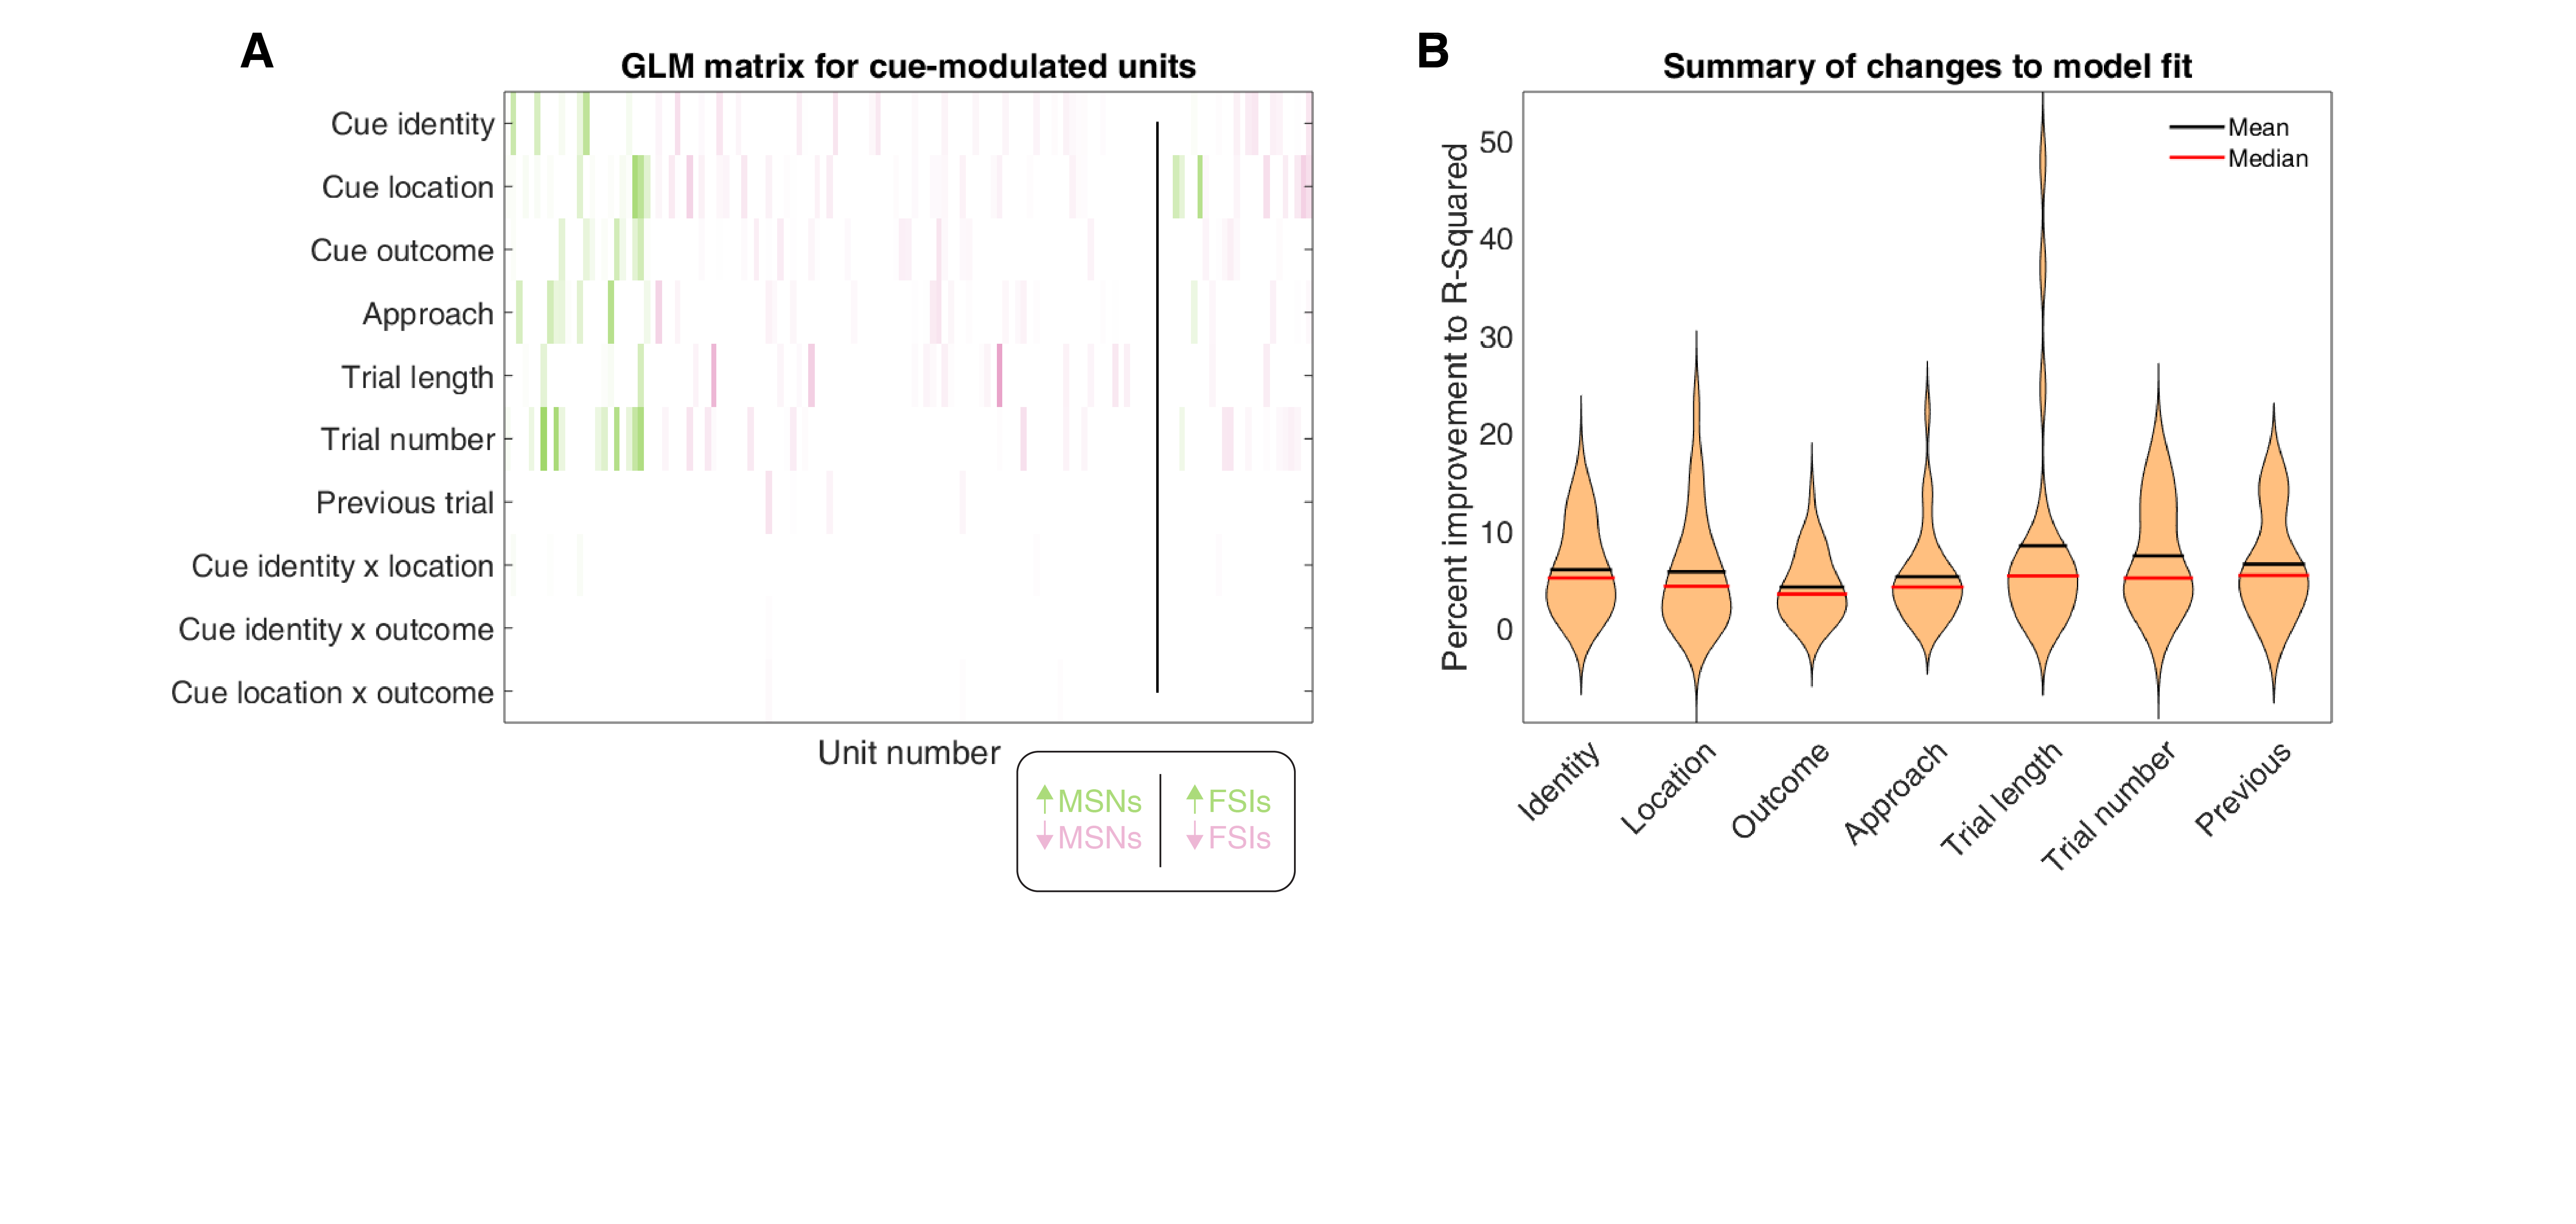
\includegraphics[width=\textwidth]{Fig 6 - GLM.png}
\caption{Summary of influence of various task parameters on cue-modulated NAc units after cue-onset.  A. GLM matrix demonstrating impact of various task parameters on NAc firing rates. A stepwise GLM was fit to each unit that showed evidence of cue modulation by a Wilcoxon signed-rank test. Each row represents a given task parameter, and each column is the influence of that task parameter on a given unit. Response variable is how much of the firing rate variance an individual predictor contributed to the model, as measured by differences in R-squared between the final model and the model minus the predictor of interest. Ordering from left to right: MSNs that increased firing in response to the cue (green, left of line), MSNs with a decreasing response (red, left of line), FSIs with an increasing response (green, right of line), FSIs with a decreasing response (red, right of line). Darker shades indicate more firing rate variance explained by a given predictor. Black line indicates separation of MSNs and FSIs. B. Violin plots demonstrating changes in R-squared values with the addition of each of the individual predictors. The mean, median, and distribution of changes in R-squared values is plotted for each of the seven task parameters used in the GLM.}
\label{fig:GLM}
\end{figure}

{\bf Population level averages reveal characteristic response profiles:}

A variety of single unit response profiles were observed around the time of cue-onset. To investigate whether these firing rate patterns were related to the cue information they represented, we looked at population level averages for units that were modulated by each feature. To do this we normalized firing activity for each unit that was modulated by a given cue feature, such as light block, then generated the cue-onset aligned population average firing rate for each of the cue features (Fig \ref{fig:pop}). This analyses revealed overall that cells that showed an increase upon cue presentation had stronger responses for the preferred cue condition (Figure \ref{fig:pop}A,C,E). Interestingly, units that were classified as decreasing in response to the cue showed a biphasic response at the population level, with a small peak at a time in alignment with entry into the arm, followed by a sustained dip after cue-onset (Figure \ref{fig:pop}B,D,F). Units that were modulated by cue identity showed a stronger increase in response to the preferred task block, as well as a higher tonic firing rate to the preferred task block, most notably in units that decreased in firing rate to the cue (Figure \ref{fig:pop}A,B). Units that were modulated by cue location showed a graded response to locations of decreasing preference, with peak firing occurring around cue-onset (Figure \ref{fig:pop}C,D). Units that were modulated by cue outcome showed a ramping of activity after cue-onset for their preferred cue type. Additionally, units that exhibited a decrease in firing in response to the cue and whose activity was modulated by cue outcome, showed a sustained discriminatory response to reward-available and reward-unavailable cues that extended beyond cue-onset (Figure \ref{fig:pop}F). Together, these visualizations of the averaged population responses revealed nuanced differences in the way NAc units are modulated by cue conditions across cue features.  

\begin{figure}[h]
\centering
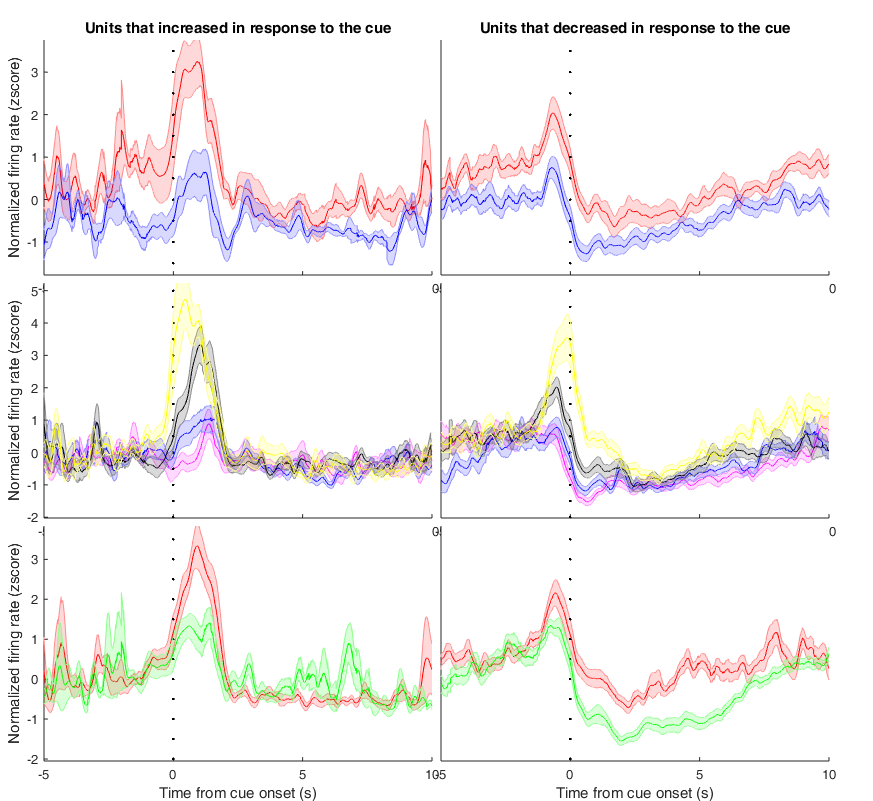
\includegraphics[width=\textwidth]{Fig 7 - Population averages.png}
\caption{Population-level averages of cue feature sensitive NAc units. A. Average smoothed normalized (z-score) activity for cue-modulated units where cue identity was a significant predictor in the GLM, aligned to cue-onset. Activity is plotted for preferred stimulus block (red) and nonpreferred stimulus block (blue). Dashed line indicates onset of cue. Lightly shaded area indicates standard error of the mean. Note larger increase to preferred stimulus block to nonpreferred stimulus block. B. Same as A but for units that decreased in firing. Note population level activity reveals cells classified as “decreasing” in response to cue show a biphasic response at the population level, with a transient increase around the time the rat starts on the arm, followed by a minimum after cue onset. Also, note the sustained difference in firing between the two blocks. C-D. Same as A-B for cue location. Activity is plotted from most preferred arm (yellow), in decreasing order to least preferred arm (black, navy blue, magneta, respectively). Note the graded response to arms of decreasing preference. E-F. Same as A-B for cue outcome. Activity is plotted for preferred expected outcome (red), and nonpreferred outcome (green). Note the larger increase to the cue representing the cell’s preferred outcome (E), and the sustained decrease to the nonpreferred outcome (F).}
\label{fig:pop}
\end{figure}

{\bf NAc units dynamically segment the task:}

Given the varied time courses and response profiles of NAc units to various aspects of the cue, the NAc may be computing a temporally evolving state value signal (Pennartz., 2011). If this is the case, then the recruitment of NAc units should vary alongside changes in the environment. To look at the distribution of responses throughout our task space and see if this distribution is modulated by cue features, we z-scored the firing rate of each unit and plotted the normalized firing rates of all units aligned to cue-onset and sorted them according to the time of peak firing rate (Figure \ref{fig:tiling}). We did this separately for both the light and sound blocks, and found a nearly uniform distribution of firing fields in task space that was not limited to alignment to the cue (Figure \ref{fig:tiling}A). Furthermore, to determine if this population level activity was similar across blocks, we also organized firing during the sound blocks according to the ordering derived from the light blocks. This revealed that while there was some preservation of order, the overall firing was qualitatively different across the two blocks. To control for the possibility that any comparison of trials would produce this effect, we did a within block comparison, comparing half of the trials in the light block against the other half. This comparison looked similar to our test comparison of sound block trials ordered by light block trials. Additionally, given that the majority of our units showed an inhibitory response to the cue, we also plotted the firing rates according to the lowest time in firing, and again found some maintenance of order, but largely different ordering across the two blocks, and the within block comparison (Figure \ref{fig:tiling}B). To further test this, we divided each block into two halves and looked at the correlation of the average smoothed firing rates across various combinations of these halves across our cue-aligned centered epoch (Table \ref{tbl3}). A linear mixed effects model revealed that within block correlations (e.g. one half of light trials vs other half of light trials) were higher and more similar than across block correlations (e.g. half of light trials vs half of sound trials), suggesting that activity in the NAc discriminates across various cue conditions. This process was repeated for cue location and cue outcome, showing that NAc segmentation of the task is qualitatively different even during those parts of the task not immediately associated with a specific cue, action, or outcome, although the within condition comparison of reward-unavailable trials was less correlated than reward-available trials, and more similar to the across condition comparisons (Figure \ref{fig:tiling}C-F). 

\begin{figure}[h]
\centering
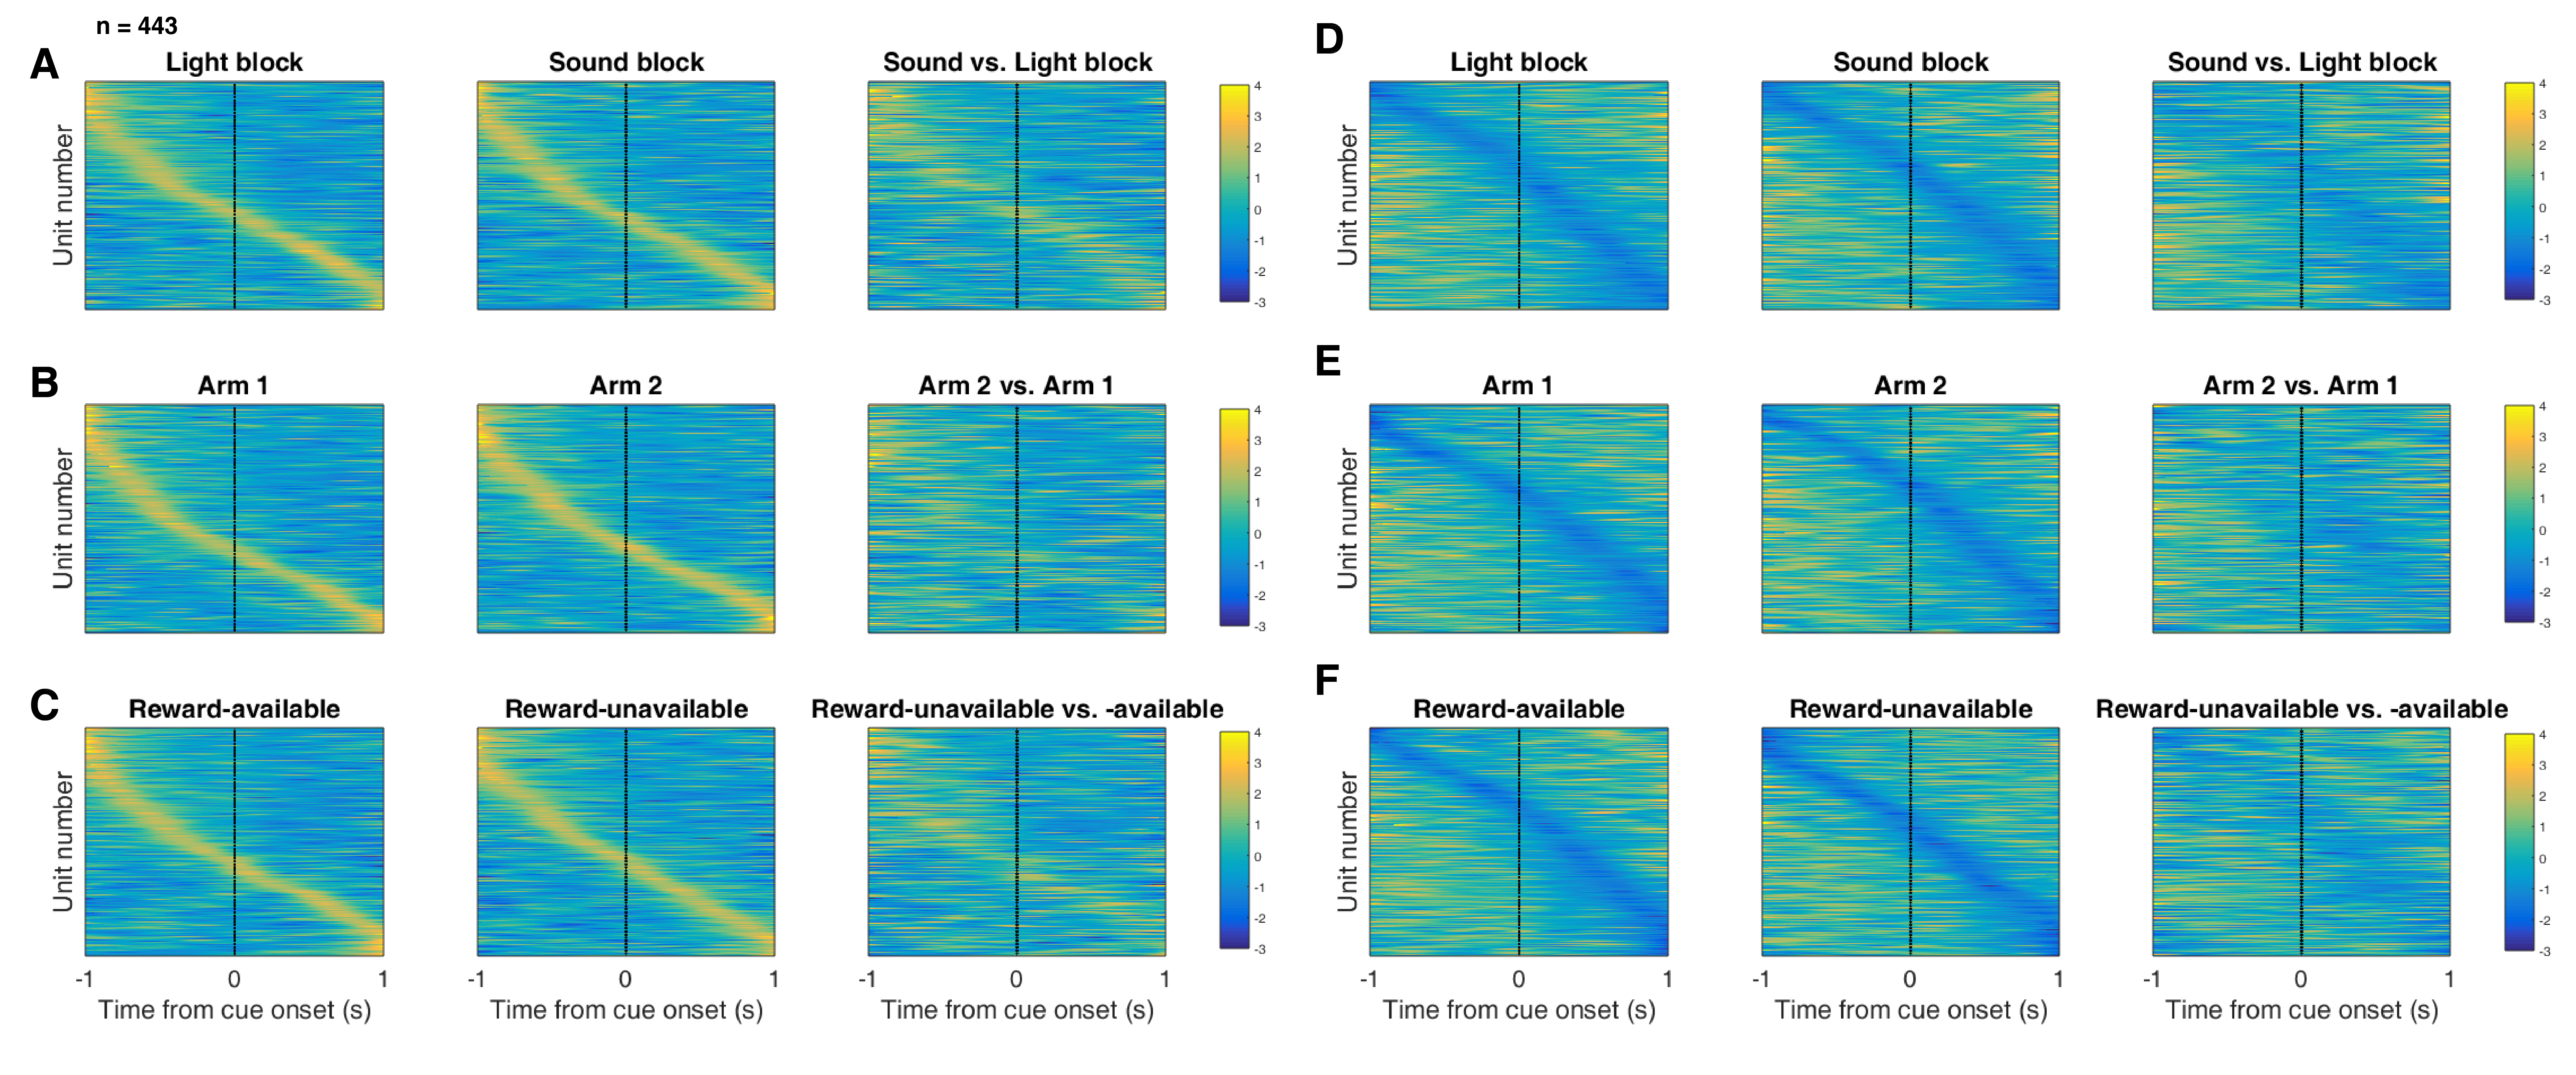
\includegraphics[height=0.7\textheight]{Fig 8 - Task tiling.png}
\caption{Distribution of NAc firing rates across time surrounding cue onset. Each panel shows normalized (z-score) firing rates for all recorded NAc units (each row corresponds to one unit) as a function of time (time 0 indicates cue onset), averaged across all trials for a specific cue type, indicated by text labels. A-C. Heat plots aligned to normalized peak firing rates. A, left: Heat plot showing smoothed normalized firing activity of all recorded NAc units ordered according to the time of their peak firing rate during the light block. Each row is a unit’s average activity across time to the light block. Dashed line indicates cue onset. Notice the yellow band across time, indicating all aspects of visualized task space were captured by the peak firing rates of various units. A, middle: Same units ordered according to the time of the peak firing rate during the sound block. Note that for both blocks, units tile time approximately uniformly with a clear diagonal of elevated firing rates. A, right: Unit firing rates taken from the sound block, ordered according to peak firing rate taken from the light block. Note that a weaker but still discernible diagonal persists, indicating partial similarity between firing rates in the two blocks. B. Same layout as in A, except that the panels now compare two different locations on the track instead of two cue modalities. As for the different cue modalities, NAc units clearly discriminate between locations, but also maintain some similarity across locations, as evident from the visible diagonal in the right panel. Two example locations were used for display purposes; other location pairs showed a similar pattern. C. Same layout as in A, except that panels now compare reward-available and reward-unavailable trials. D-F. Heat plots aligned to normalized minimum firing rates. D. Responses during different stimulus blocks as in A, but with units ordered according to the time of their minimum firing rate. E. Responses during trials on different arms as in B, but with units ordered by their minimum firing rate. F. Responses during cues signalling different outcomes as in C, but with units ordered by their minimum firing rate. Overall, NAc units "tiled" experience on the task, as opposed to being confined to specific task events only. Units from all sessions and animals were pooled for this analysis.}
\label{fig:tiling}
\end{figure}
 
\begin{table}[p]
\centering
\setlength{\tabcolsep}{1 em} % for the horizontal padding
\begin{tabular}{l c  c c c c c}

Task parameter                                 & Within condition 1        &Within condition 2        & Across conditions 1        &Across conditions 2       &Across conditions 3       &Across conditions 4\\
\hline
Cue identity       & .383         &.379          & .343          & .338          &.337        &.348\\
\hline
Cue location       & .369         &.350          & .290          & .286          & .285        &.291\\
\hline
Cue outcome       & .429        &.261          & .258        & .253          & .255        &.249\\
\hline

\end{tabular}
\caption {Firing rate correlations} \label{tbl3} 
\end{table}

{\bf Encoding of cue features is maintained until outcome:}

In order to be useful for reinforcement learning, a trace of the cue must be maintained until the outcome to link the outcome to the outcome-predictive cue. To test whether representations of cue features were maintained post-approach until the outcome was revealed, we fit a GLM to the post-approach firing rates of cue-modulated units aligned to the time of nosepoke into the reward receptacle. This analysis showed that a variety of units still discriminated firing according to various cue features, but not other task parameters, showing that NAc activity discriminates various cue conditions well into a trial (Table \ref{tbl4}, Figure \ref{fig:NP_GLM}). Fitting a GLM to all recorded units...*Jimmie finish this* (data not shown). Population level averages for units that increased to cue-onset showed a ramping up of activity that peaked upon nosepoke, whereas units that decreased to cue-onset showed a gradual reduction of firing activity that reached a minimum upon nosepoke (Figure \ref{fig:NP_pop}). Additionally, a peak is seen for preferred cue outcome in decreasing units at 1 second post cue-onset when reward was received, demonstrating an integration of expected and received reward (Figure \ref{fig:NP_pop}F). Furthermore, aligning normalized peak firing rates to nosepoke onset, revealed a clustering of responses around reward receipt for all cue conditions where the rat would have received reward (Figure \ref{fig:NP_tiling}). To determine whether coding of cue features was maintained after the outcome was revealed, a GLM was fit to the firing rates of cue-modulated units at the time of reward receipt, during which the cue was still present. Fitting a GLM revealed 10 units (8\%) where cue outcome accounted for an average of 32\% of firing rate variance (data not shown). However, an absence of cue identity or cue location coding was observed, suggesting that the NAc does not maintain a representation of these cue features once the rat receives behavioral feedback for its decision.

\begin{table}[p]
\centering
\setlength{\tabcolsep}{1 em} % for the horizontal padding
\begin{tabular}{l c  c c c c}

Task parameter                                 & Total        & MSN (increasing)        & MSN (decreasing)        &FSI (increasing)        &FSI (decreasing)\\
\hline
All cells                       & 443        & 155         & 216          & 27          & 45\\
\hline
Cue modulated                       & 133         &24          &85          & 6          &18\\
\hline
Cue identity       & 66         &14          & 36          & 2          &14\\
\hline
Cue location       & 66         &14          & 40          & 3          & 9\\
\hline
Cue outcome       & 42        & 8          & 29        & 0          & 5\\
\hline
Trial length       & 0        & 0         & 0         & 0         & 0\\
\hline
Trial number       & 0         & 0          & 0         & 0          & 0\\
\hline
Recent trial history       & 0         & 0          &0          & 0          & 0\\
\hline
Cue x cue interactions       & 0         &0          & 0          & 0          & 0\\
\hline
Cue x behavior interactions       & 0         & 0          & 0          & 0          & 0\\
\hline

\end{tabular}
\caption {Cells from nosepoke GLM} \label{tbl4} 
\end{table}

\begin{figure}[h]
\centering
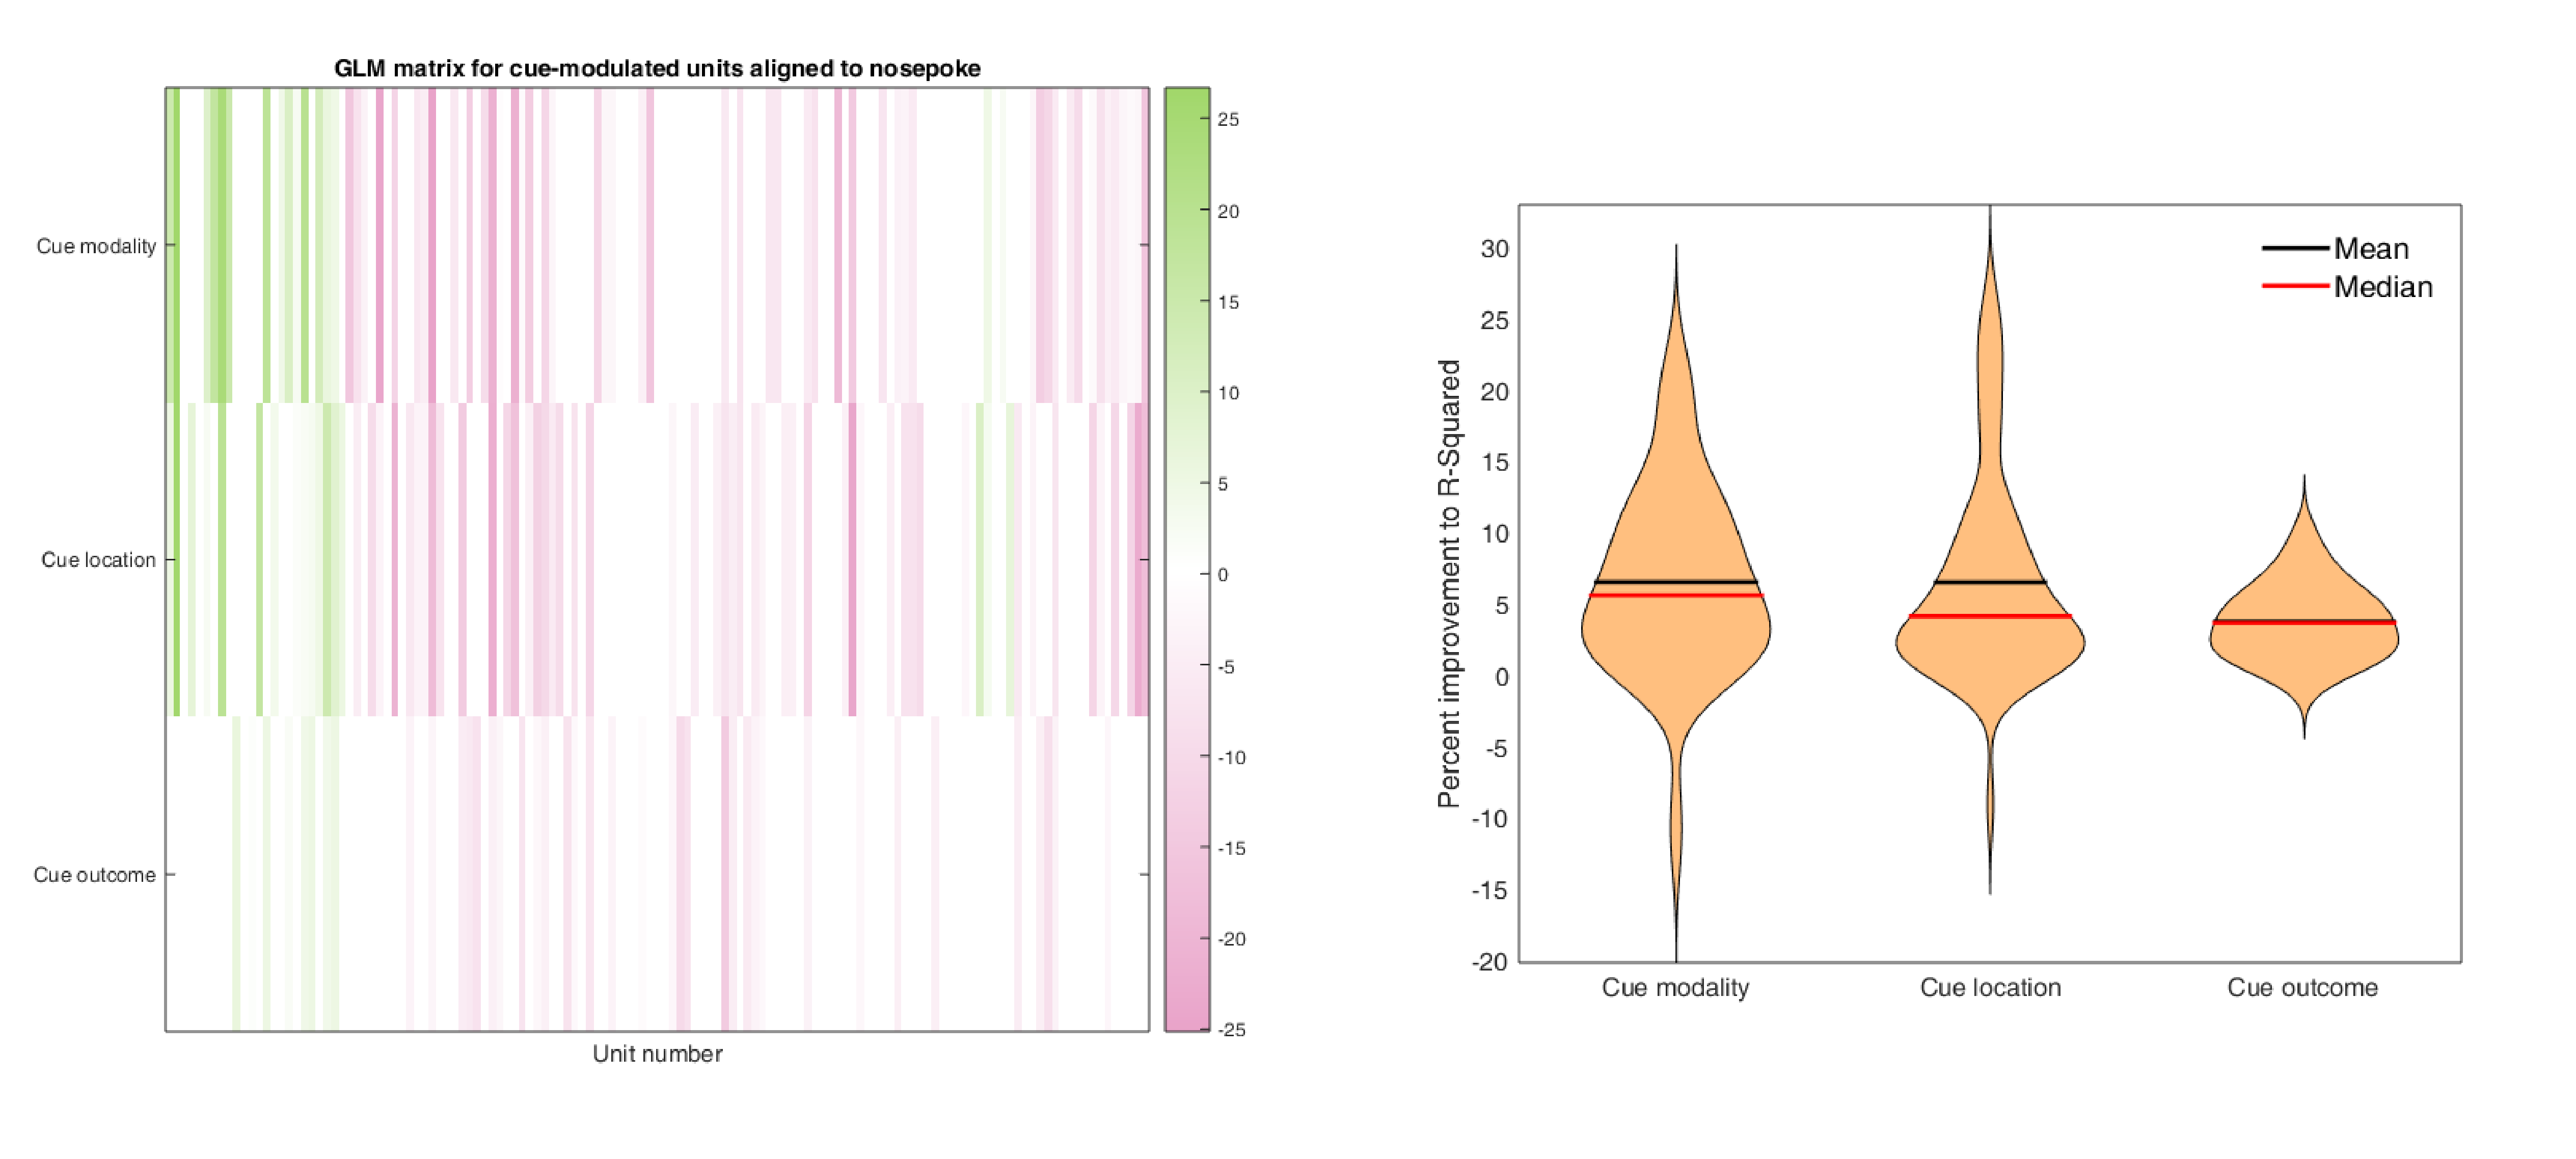
\includegraphics[width=\textwidth]{Fig 9 - NP GLM.png}
\caption{Summary of influence of various task parameters of cue-modulated NAc units during nosepoke. A. GLM matrix demonstrating impact of various task parameters on NAc firing rates. A stepwise GLM was fit to each unit that showed evidence of cue modulation by a Wilcoxon signed-rank test. Each row represents a given task parameter, and each column is the influence of that task parameter on a given unit. Response variable is how much of the firing rate variance an individual predictor contributed to the model, as measured by differences in R-squared between the final model and the model minus the predictor of interest. Ordering from left to right: MSNs that increased firing in response to the cue (green, left of line), MSNs with a decreasing response (red, left of line), FSIs with an increasing response (green, right of line), FSIs with a decreasing response (red, right of line). Darker shades indicate more firing rate variance explained by a given predictor. Black line indicates separation of MSNs and FSIs. B. Violin plots demonstrating changes in R-squared values with the addition of each of the individual predictors. The mean, median, and distribution of changes in R-squared values is plotted for each of the three task parameters that were significant predictors in the GLM.}
\label{fig:NP_GLM}
\end{figure}

\begin{figure}[h]
\centering
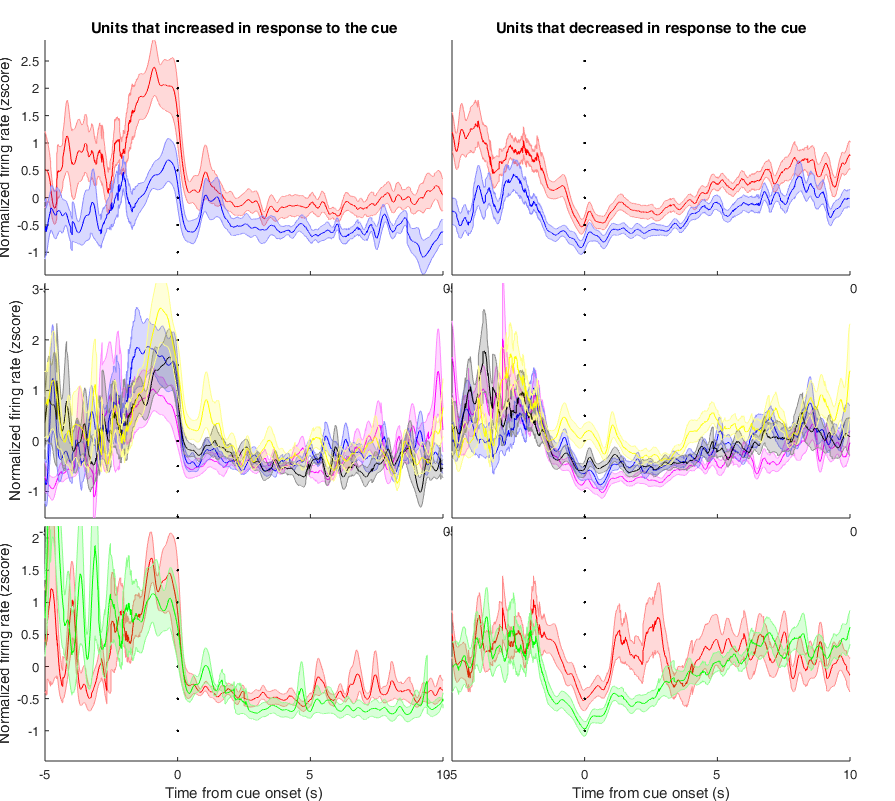
\includegraphics[width=\textwidth]{Fig 10 - NP population averages.png}
\caption{Population-level averages of cue feature sensitive NAc units during a nosepoke. A. Average smoothed normalized activity for cue-modulated units where cue identity was a significant predictor in the GLM, aligned to nosepoke with reward delivery occurring 1 s after nosepoke. Activity is plotted for preferred stimulus block (red) and nonpreferred stimulus block (blue). Dashed line indicates nosepoke. Lightly shaded area indicates standard error of the mean. Note larger increase leading up to nosepoke to preferred stimulus block to nonpreferred stimulus block. B. Same as A but for units that decreased in firing. Note the sustained difference in firing between the two blocks. C-D. Same as A-B for cue location. Activity is plotted from most preferred arm (yellow), in decreasing order to least preferred arm (black, navy blue, magneta, respectively). Note the subtle but graded response to arms of decreasing preference. E-F. Same as A-B for cue outcome. Activity is plotted for preferred expected outcome (red), and nonpreferred outcome (green). Note the peak after reward receipt for preferred outcome in decreasing cells (F).}
\label{fig:NP_pop}
\end{figure}

\begin{figure}[h]
\centering
\includegraphics[width=\textwidth]{Fig 11 - NP task tiling.png}
\caption{Distribution of NAc firing rates across task space during approach trials. Each panel shows normalized firing rates for all recorded NAc units (each row corresponds to one unit) as a function of time (time 0 indicates nosepoke), averaged across all approach trials for a specific cue type, indicated by text labels. A, left: Heat plot showing smoothed normalized firing activity of all recorded NAc units ordered according to the time of their peak firing rate during the light block. Each row is a unit’s average activity across time to the light block. Dashed line indicates nosepoke with reward delivery occurring 1 s after nosepoke for reward-available trials. Notice the yellow band across time, indicating all aspects of visualized task space were captured by the peak firing rates of various units. A, middle: Same units ordered according to the time of the peak firing rate during the sound block. Note that for both blocks, units tile time approximately uniformly with a clear diagonal of elevated firing rates, and a clustering around reward receipt. A, right: Unit firing rates taken from the sound block, ordered according to peak firing rate taken from the light block. Note that a weaker but still discernible diagonal persists, indicating partial similarity between firing rates in the two blocks. B: Same layout as in A, but with units ordered according to the time of their minimum firing rate. C: Same layout as in A, except that the panels now compare two different locations on the track instead of two cue modalities. As for the different cue modalities, NAc units clearly discriminate between locations, but also maintain some similarity across locations, as evident from the visible diagonal in the right panel. Two example locations were used for display purposes; other location pairs showed a similar pattern. D: As for C, but with units ordered by their minimum firing rate. E: Same layout as in A, except that panels now compare reward-available and reward-unavailable trials. Notice the absence of a cluster of tiling around reward receipt for reward-unavailable trials. F: As for A, but with units ordered by their minimum firing rate. Overall, NAc units "tiled" experience on the task, as opposed to being confined to specific task events only. Units from all sessions and animals were pooled for this analysis.}
\label{fig:NP_tiling}
\end{figure}

\section*{Discussion}

The present study found evidence for coding of multiple identifying features of motivationally relevant stimuli in addition to expected outcome; the sensory modality of the presented cue, as well at its physical location within the track, and that this coding was still present on approach trials when the rat nosepoked. Furthermore, this coding was both independent, and intermixed across cue features and behavioral measures. Coding at the population level revealed qualitatively distinct comparison profiles across cue features, such as cells that encoded cue modality tended to sustain the discriminatory firing outside of cue presentation, while a subset cells that discriminated rewarded from unrewarded cues maintained this discrimination until after reward receipt. Across all recorded cells, a tiling of task structure was observed such that all points within our analyzed task space was accounted for by the ordered peak firing rates of all cells, and this tiling differed between various conditions with a cue feature, such as light versus sound blocks. Cells that discriminated across blocks were not simply due to drifting of the signal across trials, as cells that showed a drift in firing between the first and second half within a block were excluded from the analysis. Furthermore, even though actions were stereotyped during correct trials, such that the rat always turned left at the decision point to approach for reward, and right to skip the receptacle and initiate the next trial, cells that were modulated by the expected value of the cue maintained their specific firing patterns even during error trials where the rat turned left after presentation of the unrewarded cue, suggesting that these signals did not represent action values. Additionally, NAc signals have been shown to be modulated by response vigor, to detangle this from our results we included the trial length as a predictor in our GLMs, and found cells with correlates independent of trial length.

{\bf Cue modality:}  

Our finding that NAc units can discriminate between cues from different sensory modalities expands upon an extensive literature examining neural correlates of conditioned stimuli. Perhaps the most comparable work in rodents comes from a study that found distinct coding for an odor when it predicted separate but equally valued rewards (Cooch). The present work is complementary to this as it shows that NAc cells have representations of identifiable aspects of the cue itself, in addition to the reward it predicts. Another study paired separate cues with appetitive or aversive outcomes, and found separate populations of cells that encode each cue, with many switching selectivity after reversal of the associations between the cues and outcomes, providing evidence that the NAc encodes the biological significance of stimuli. Once again, our study was different as we recorded neural responses to distinct cues encoding the same anticipated outcome, suggesting that even when the biological relevance of these stimuli is similar, the NAc dissociates their representations at the level of the single-unit (Setlow), although this doesn’t explain the difference in population averaged firing rate for the epochs when the cue is not present. Another possibility is that these modality specific cells were encoding the context, rule, or sequence within a session as some cells responded similar for both rewarded and unrewarded cues within a block. This interpretation is in alignment with a recent paper from the primate realm that recorded NAc responses during the Wisconsin Card Sorting Task (WCST), a common set-shifting task used in both the laboratory and clinic, and found cells that preferred firing to stimuli when a certain rule, or rule category was currently active (Sleezer). Indeed, an encoding of the current strategy could be an explanation as to why a sustained difference in population averaged firing was seen across stimulus blocks, as well as a potential explanation for the differentially tiling of task structure across blocks in the current study. Further support for a modulation of NAc responses by strategy comes from an fMRI study that examined BOLD levels during a set-shifting task (FitzGerald et al., 2014). In this task, participants learned two sets of stimuli-reward contingencies, a visual set and auditory set. During testing they were presented with both simultaneously, and the stimulus dimension that was relevant was periodically shifted between the two. Here, they found that bilateral NAc activity reflected value representations of whatever the currently relevant stimulus dimension was, and not the irrelevant stimulus. The current finding of separate, but overlapping, populations of cells encoding cue modality and expected value, suggests that the fMRI finding is generated by the combined activity of several different functional cell types.

A caveat of the current study is that rats were never presented with both sets of cues simultaneously, and thus never had to switch strategies, although extrapolating the data from the primate study, suggests that the activity of the cue modality cells would be modulated by relevance. Keeping along this theme, the current data set is unable to identity precisely what the modality-sensitive neurons were encoding, that is were they tracking representations of stimulus identity, a preferred context, or even a macroscale representation of progress through the session. Furthermore, their relevance for ongoing behavior is also uncertain. NAc core lesions have been shown to impair shifting between different behavioral strategies, and it is possible that selectively silencing the cells that prefer responding for a given modality or rule would impair performance when the animal is required to use that information, or artificial enhancement of those cells would cause them to use the rule when it is the inappropriate strategy.

{\bf Encoding of position:} 

Our finding that cue-evoked activity was modulated by cue location sides with some of the literature (Lavoie, 1994; Tabuchi, 2000; Strait, 2016). An alternative explanation for a pure spatial representation, is that these are task segmentation correlates, keeping track of where in the task the rat is. A previous non-human primate paper has shown that when reward is contingent upon completion of a series of trials, separate populations of NAc neurons signal the start of a schedule, subsequent trials in the schedule, and the first trial in extended schedules (Shidara et al., 1998). This signalling of position within a sequence has been observed in subsequent studies, and it is possible that the our rats were keeping track of which specific arm they were in as part of a sequence of arms, and not just strictly a spatial representation (Mulder, 2004 and 2005; Khamassi et al., 2008; Berke, 2009). Also, given that our task is pseudo-random, it is possible that the rats learned which cue to anticipate, and the neural activity could reflect this. However, this is unlikely as including a ‘previous trial’ variable in the analysis did not explain a significant amount of firing rate variance in response to the cue for the vast majority of cells..

{\bf Mixed selectivity:} 

Several other papers have reported unit profiles that integrate different task-related variables. These papers report integrated coding between expected value and subsequent motor responses, expected value and identity of a reward, and a combination of spatial-, movement-, and reward-related features (Roesch, Lavoie, Cooch). However, our study is the first to show mixed selectivity among identifying features of a cue and expected outcome or behavior. The presence of mixed selectivity responses confers a larger number of input-output relationships that are available to a given neuron. A possible functional consequence of this attribute of NAc units, is the combination and transformation of various motivationally relevant features into a signal informing downstream decoders such as the ventral pallidum about appropriate behaviors in obtaining motivationally relevant goals and biasing action selection towards these behaviors. 

Mixed selectivity in the NAc could be a consequence of synaptic integration from a variety of anatomically distinct inputs, as seen in experiments examining the convergence of various NAc afferents at the level of synaptic transmission and stimulation-induced firing (Goto and Grace 2008). In one such experiment it was shown that NAc cells that responded to stimulation of either the fornix, amygdala, or PFC, typically responded to stimulation from all inputs (O’Donnell and Grace, 1995). Furthermore, an interaction between these inputs was observed such that PFC stimulation failed to elicit spiking in the NAc neurons unless they were in a depolarized UP-state, a state induced by hippocampal stimulation and was dependent on an intact fornix. Hippocampal-induced suppression of other inputs has also been observed for the BLA (Mulder et al., 1998). Recently, it has also been shown that train stimulation of PFC afferents reduces hippocampal-evoked NAc responses, suggesting that there is competition between various inputs (Calhoon and O’Donnell, 2013). These studies suggest that the integration of the variables we saw could be the result of this gating observed in behaviorally-independent preparations. However, given that we did not systematically manipulate these various limbic and cortical afferents, comments on the anatomical origins of the observed mixed selectivity responses are speculative at this point.

Integrating cue identity and value, as seen modestly in the present study, could be one neural instantiation of how value is associated with the appropriate predictive stimuli (credit assignment), keeping in mind that value encoding is distributed, redundantly in some aspects, across various structures (Hayden Nat Neuro opinion). Indeed, lesions of the NAc impair the ability to learn changes in reward value or identity in an unblocking experiment, as well as disrupting dopamine RPEs generated by modification of timing of reward (McDannald 2011, Takahashi 2016). Would be interesting to see if uncoupling the integrated coding of stimulus features and predictive properties of a cue has an effect on the ability of a rat to use reward-predictive cues to pursue the associated reward.

{\bf Tiling of task structure:}

Additionally, we found that the population of recorded units had a relatively uniform distribution of firing fields within our task space, similar to what has been reported previously (Shidara, 1998; Berke, 2009; Lansink, 2012). Uniquely, we found that this representation differed according to whether the rat was currently engaged in the light or sound block, suggesting that this could be a possible neural correlate for encoding the currently relevant strategy in the NAc. It has been previously shown that during progress through a predictable trial series, neurons represented state value of cue (Shidara 1998), and that single-unit responses allowed the monkey to know how it was progressing throughout the task. Likewise, the tiling we saw could be a consequence of upstream cortical or limbic inputs informing the striatum of the current task rules. Another possibility is that the NAc not only pays attention to progress throughout a task within a trial, but also higher-order task information, like blocks. Furthermore, dopamine levels in the NAc fluctuate through a trial, and it is possible that the observed tiling could be a NAc-representation of state value related to this temporally evolving dopamine signal. Future experiments should monitor this mapping of task structure during the application of dopamine antagonists. Finally, the presence of functional correlates not evident when looking at single-unit responses time-locked to salient task events emphasizes the need to employ ensemble level analyses across all aspects of a task.

\bibliography{vStrCueCoding}
\end{document}
